\documentclass[a4paper]{article}
\usepackage[12pt]{extsizes}
\usepackage[utf8]{inputenc}
\usepackage[russian]{babel}
\usepackage{setspace}
\usepackage{amsmath}
\usepackage[left=10mm, top=15mm, right=10mm, bottom=15mm, nohead, footskip=10mm]{geometry} 
\usepackage{wrapfig}
\usepackage[pdftex]{graphicx}
\usepackage{indentfirst}
\usepackage[outdir=./pictures/]{epstopdf}
\graphicspath{{pictures/}{../handle/SLIT6/}{../handle/SLIT7/}}
\epstopdfsetup{outdir=./pictures/}
\DeclareGraphicsExtensions{.eps,.pdf,.png,.jpg}
\begin{document}
\setcounter{page}{0} 
\begin{titlepage}
\begin{center}
\large{\textbf{МОСКОВСКИЙ ГОСУДАРСТВЕННЫЙ УНИВЕРСИТЕТ\\ИМЕНИ М.В. ЛОМОНОСОВА}}\\
\hfill\break
\normalsize{ФИЗИЧЕСКИЙ ФАКУЛЬТЕТ}\\
\hfill\break
\normalsize{ГОСУДАРСТВЕННЫЙ АСТРОНОМИЧЕСКИЙ ИНСТИТУТ ИМЕНИ П.К. ШТЕРНБЕРГА}\\
\hfill\break
\hfill\break
\hfill\break
\hfill\break
\hfill\break
\hfill\break
\hfill\break
\hfill\break
\hfill\break
\hfill\break
\Large{\textbf{ОПРЕДЕЛЕНИЕ ЭФФЕКТИВНОСТИ ИНФРАКТРАСНОЙ КАМЕРЫ\\ПРИ РАБОТЕ В СПЕКТРАЛЬНОМ РЕЖИМЕ}}\\
\hfill\break
\normalsize{(Н.А. МИТИЧКИН, И.А. ОРЛОВ)}\\
\hfill\break
\normalsize{РУКОВОДИТЕЛЬ: А.М. ТАТАРНИКОВ}\\
\end{center}
\hfill\break
\hfill\break
\hfill\break
\hfill\break
\hfill\break
\hfill\break
\hfill\break
\hfill\break
\hfill\break
\hfill\break
\hfill\break
\hfill\break
\hfill\break
\hfill\break
\hfill\break
\hfill\break 
\hfill\break
\hfill\break
\hfill\break
\begin{center}
Кавказская горная обсерватория ГАИШ МГУ имени М.В. Ломоносова, июль 2018 г.
\end{center}
\thispagestyle{empty}
\end{titlepage}
\newpage
\tableofcontents
\newpage
\section{Введение}
\begin{wrapfigure}[12]{r}{0.40\linewidth} 
\vspace{-4ex}
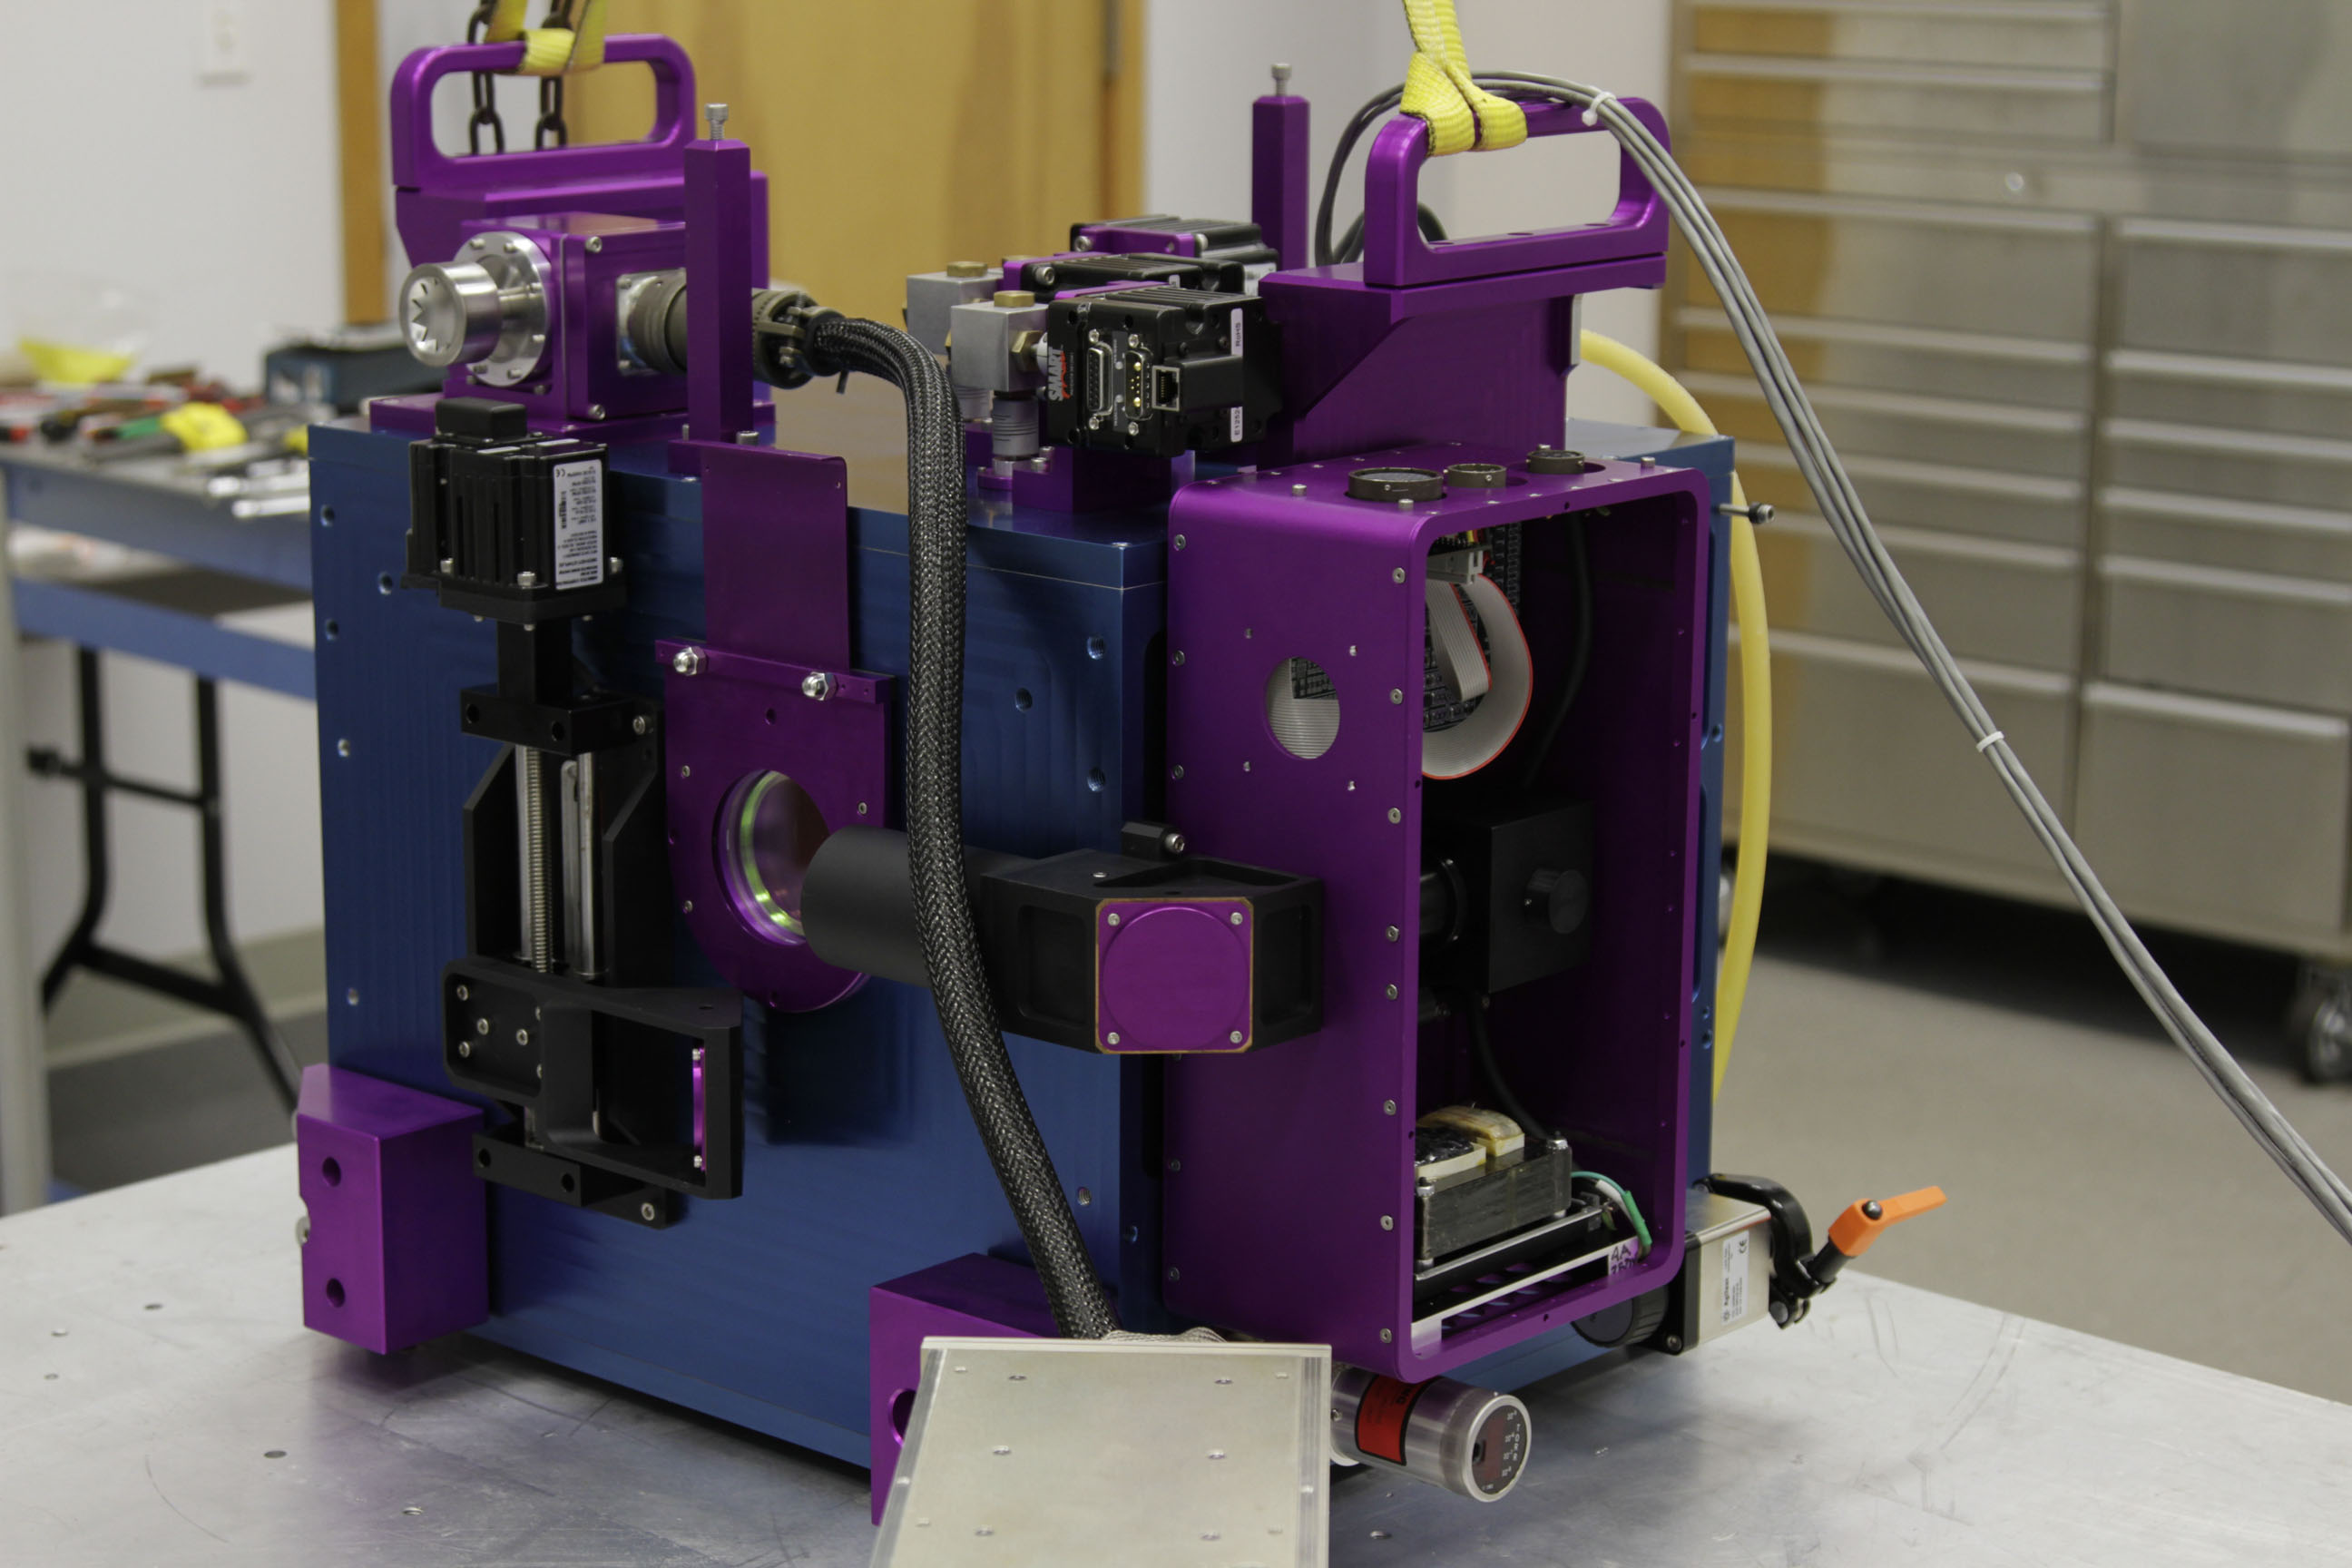
\includegraphics[width=\linewidth]{11}
\caption{Внешний вид устройства ASTRONIRCAM.}
\label{fig:1}
\end{wrapfigure}
Основной задачей данной работы является определние эффективности инфракрасной камеры прибора ASTRONIRCAM при работоте в спектральном режиме.

ASTRONIRCAM - это криогенно-охлаждае-мый щелевой спектрограф на спектральную область 1-2.5 мкм, установленный в фокусе Нэсмита\footnote{Система Нэсмита - это трехзеркальная модификация системы Кассегрена, в которой внутри трубы телескопа между главным и вторичным зеркалами установлено диагональное зеркало для отбрасывания изображения вбок. Таким образом, фокус телескопа, называемый фокусом Несмита, находится сбоку трубы. Такая оптическая схема позволяет нагружать телескоп громоздким наблюдательным оборудованием, без разбалансирования трубы.} 2.5-м телескопа Кавказской горной обсерватории ГАИШ МГУ имени М.В. Ломоносова. При работе в спектроскопическом режиме прибор позволяет получать спектры протяжённых и точечных астрономических объектов с разрешающей силой $R = \dfrac{\lambda}{\delta\lambda}\leq 1200$.

Подробнее про принцип и особенности работы прибора ASTRONIRCAM можно прочесть в \cite{Sulsky1994}.

\hfill\break

\section{Наблюдения}
Первым этапом выполнения задачи являлось получение спектров исследуемой звезды HIP85382 спектрального класса A0V. Наблюдения проводились с использованием двух спектральных  щелей STIT6 и SLIT7 в фотометрических фильтрах: YOS, JOS, H и K. Результаты наблюдений представлены на Рис. 2 и Рис. 3.
\begin{figure}[h]
\begin{minipage}[h]{0.5\linewidth}
\center{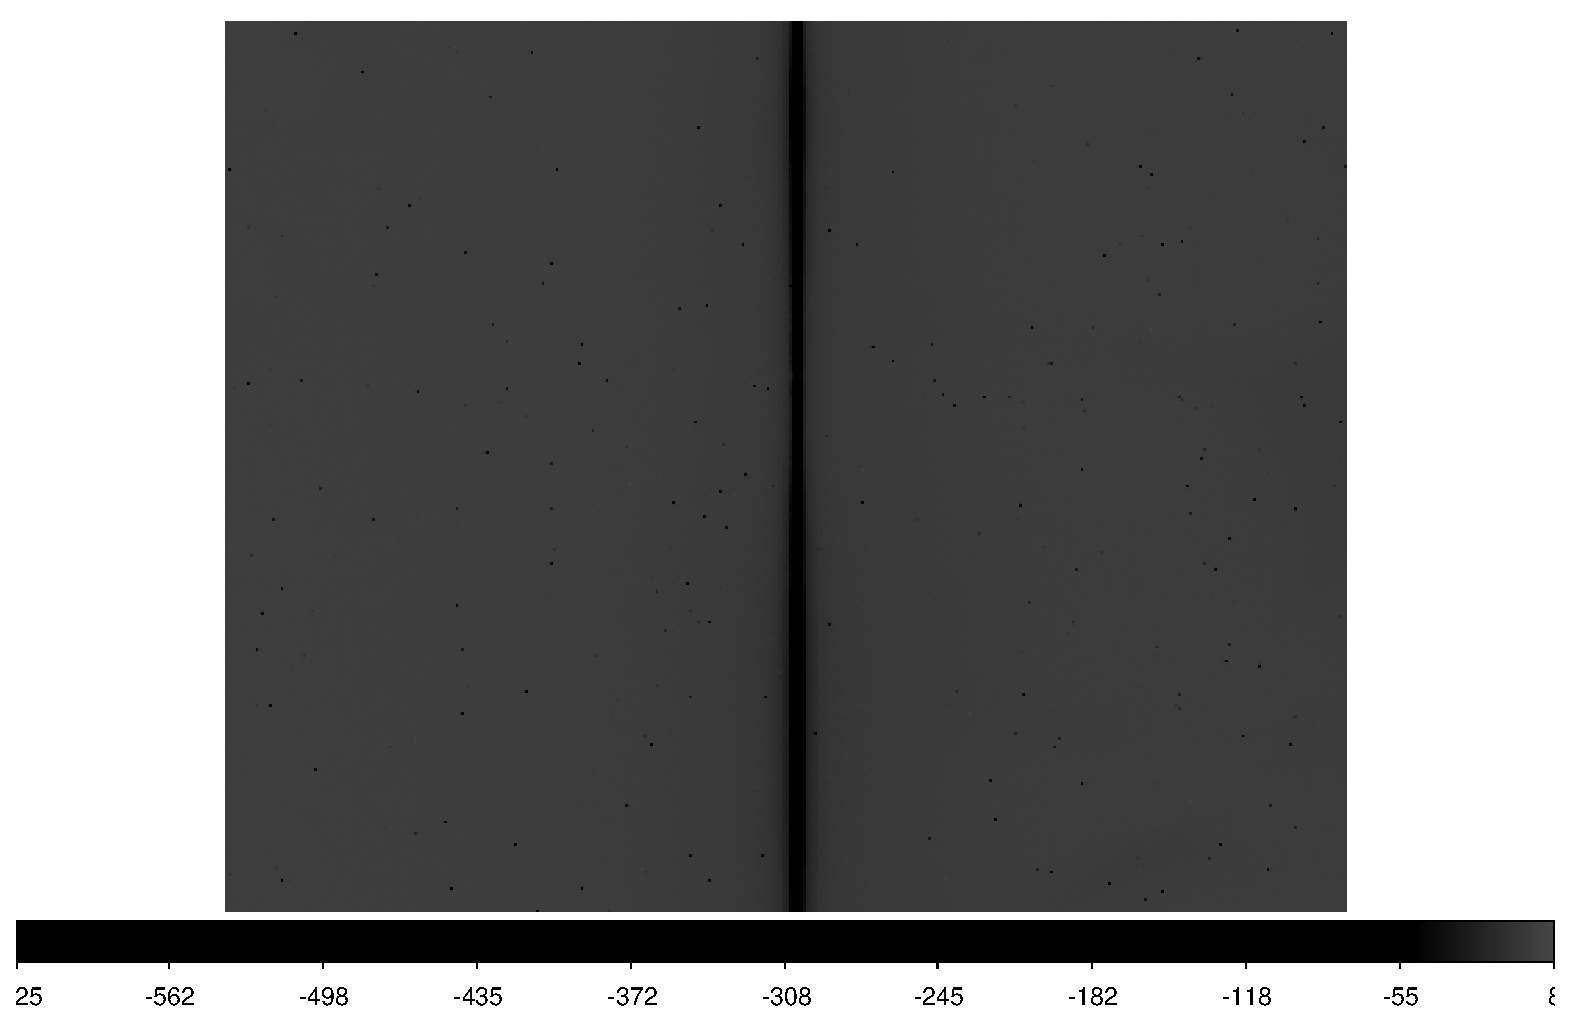
\includegraphics[width=0.75\linewidth]{SLIT6_Y} \\ фильтр YOS}
\end{minipage}
\begin{minipage}[h]{0.5\linewidth}
\center{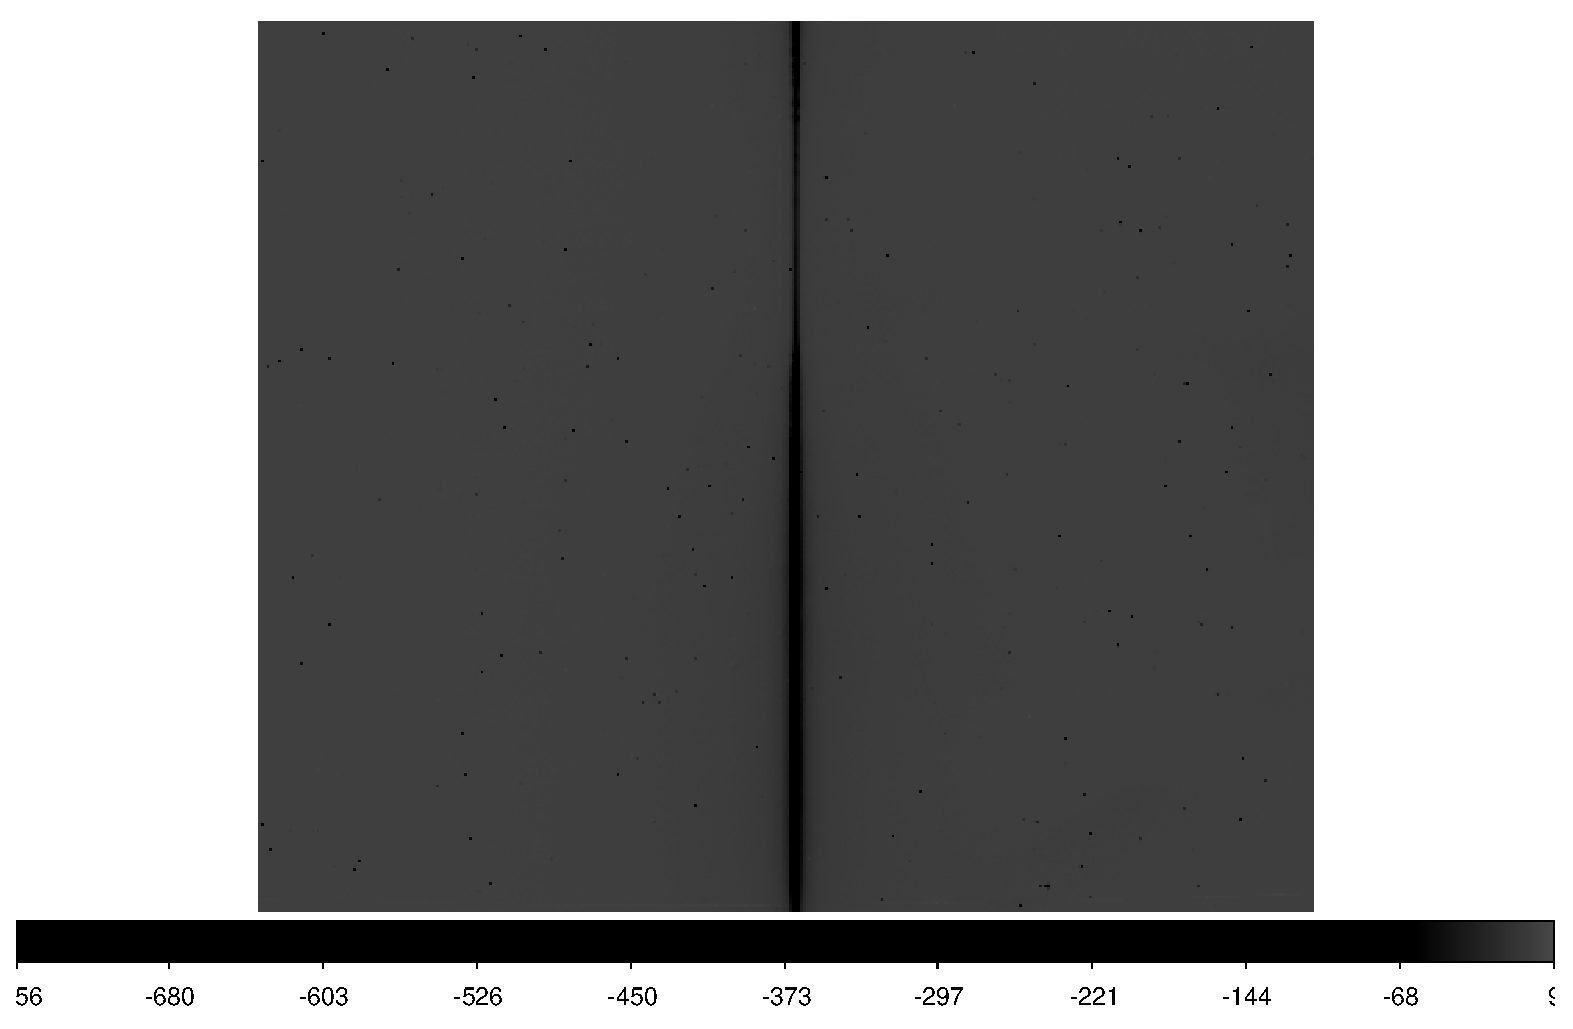
\includegraphics[width=0.75\linewidth]{SLIT6_J} \\ фильтр JOS}
\end{minipage}
\begin{minipage}[h]{0.50\linewidth}
\center{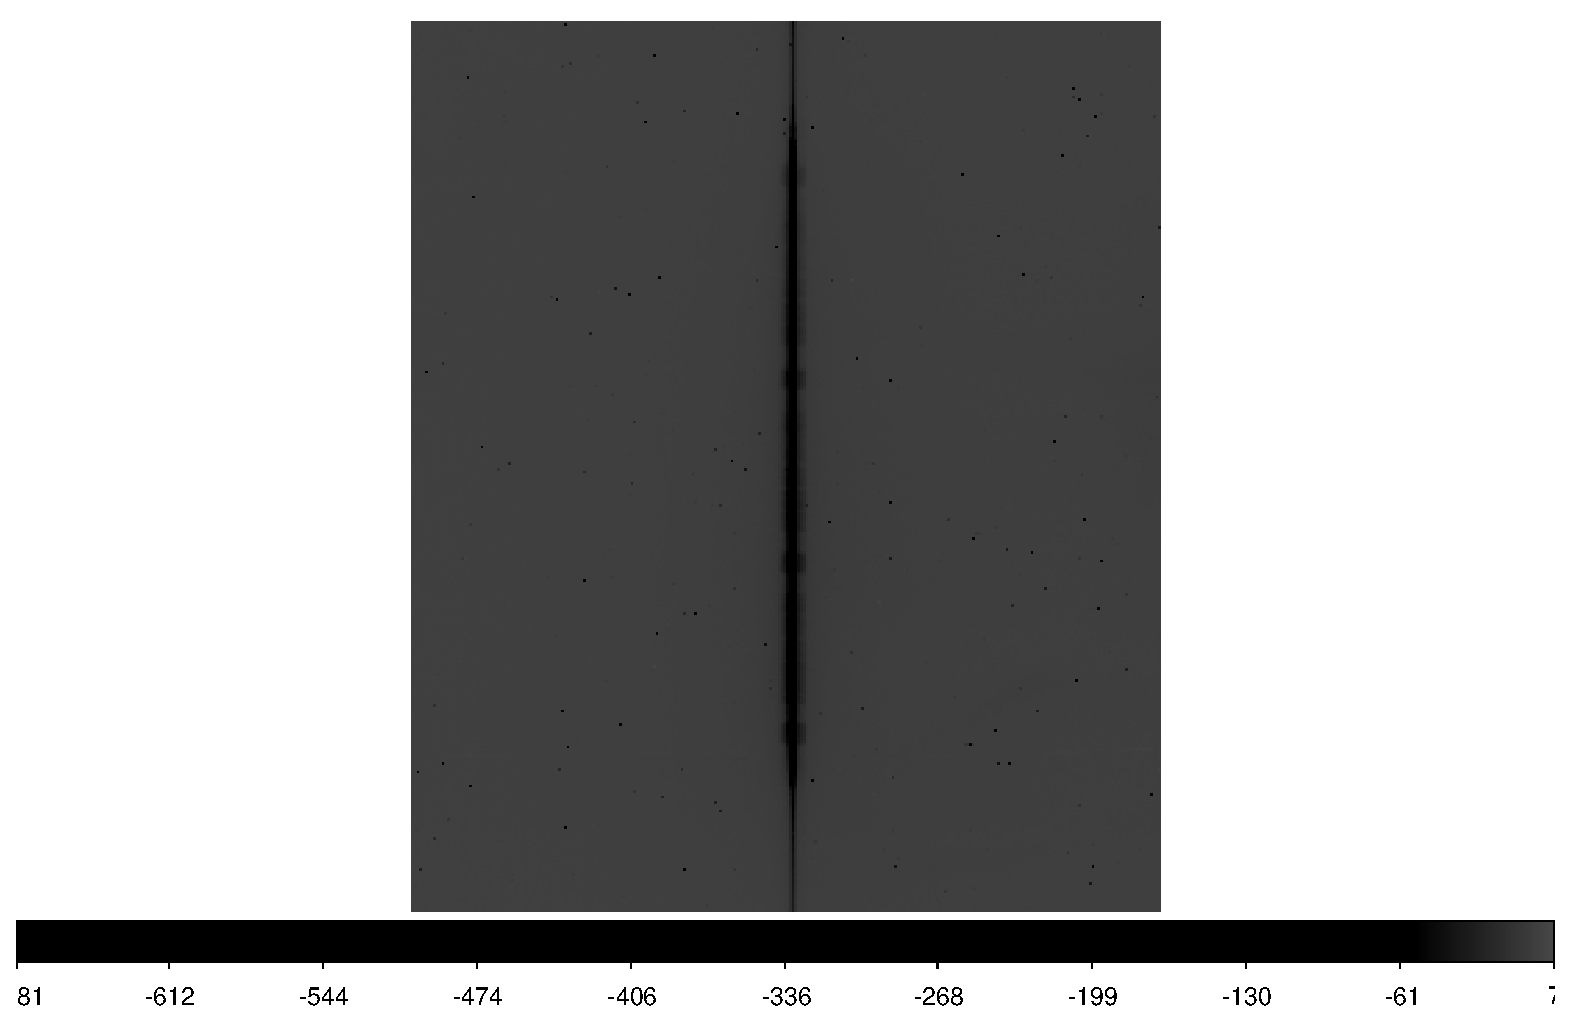
\includegraphics[width=0.75\linewidth]{SLIT6_H} \\ фильтр H}
\end{minipage}
\begin{minipage}[h]{0.50\linewidth}
\center{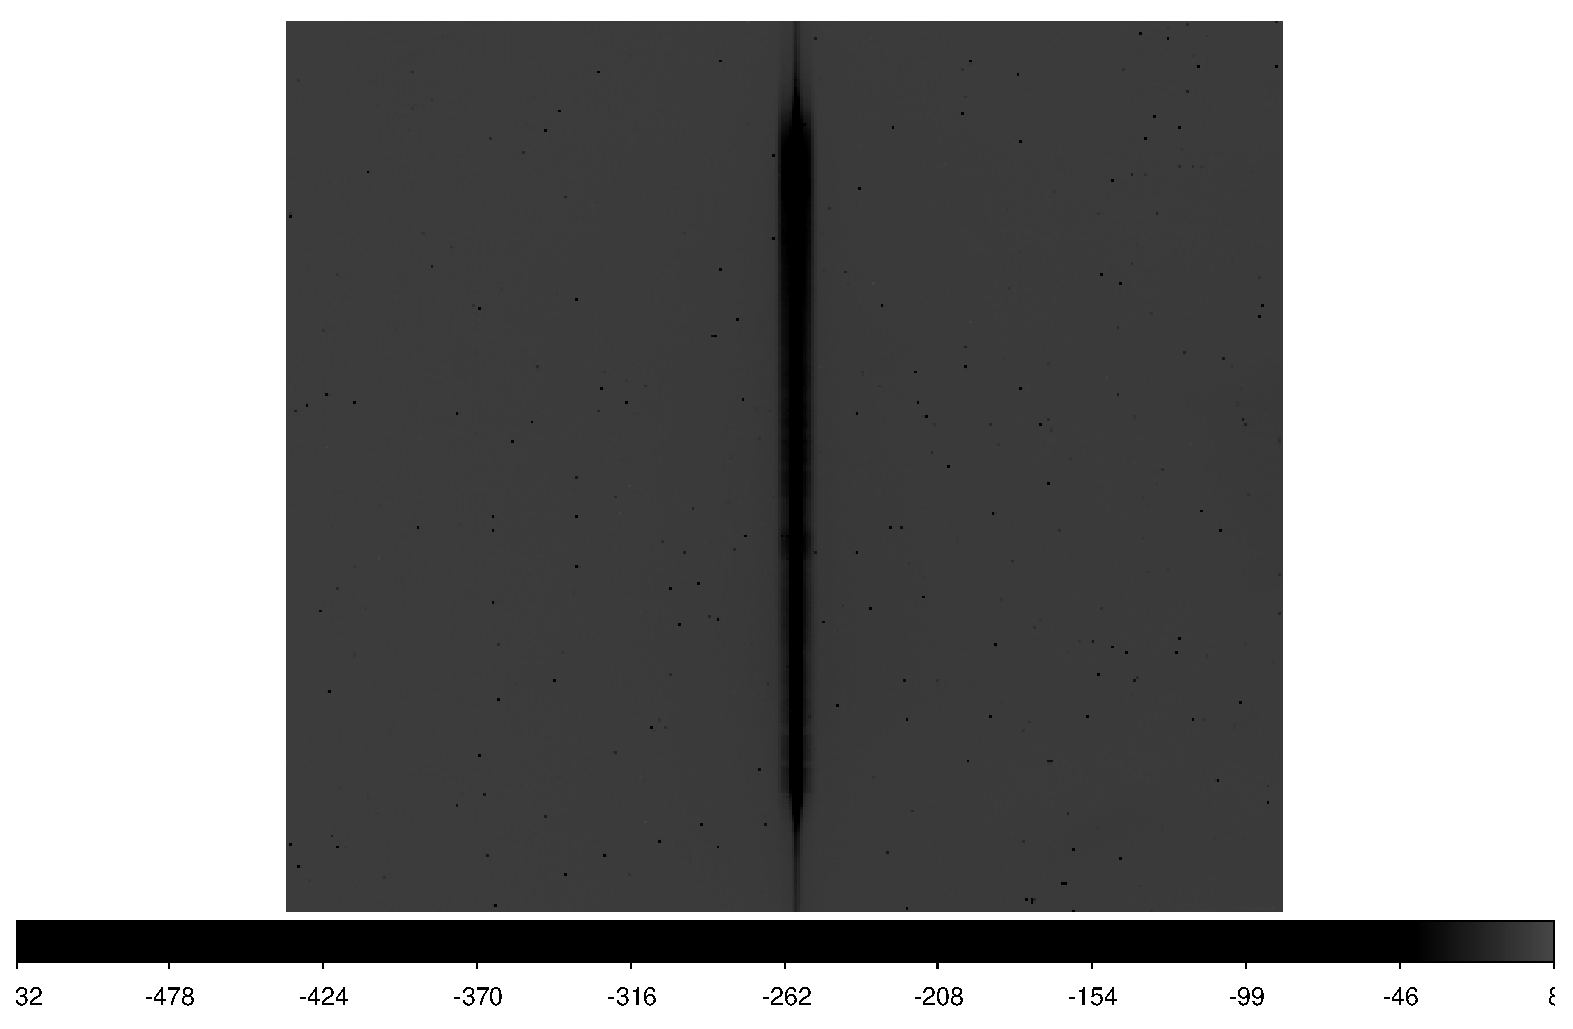
\includegraphics[width=0.75\linewidth]{SLIT6_K} \\ фильтр K}
\end{minipage}
\caption{Спектры звезды с использованием спектральной щели SLIT6.}
\label{ris:image1}
\end{figure}
\hfill\break
\begin{figure}[h]
\begin{minipage}[h]{0.50\linewidth}
\center{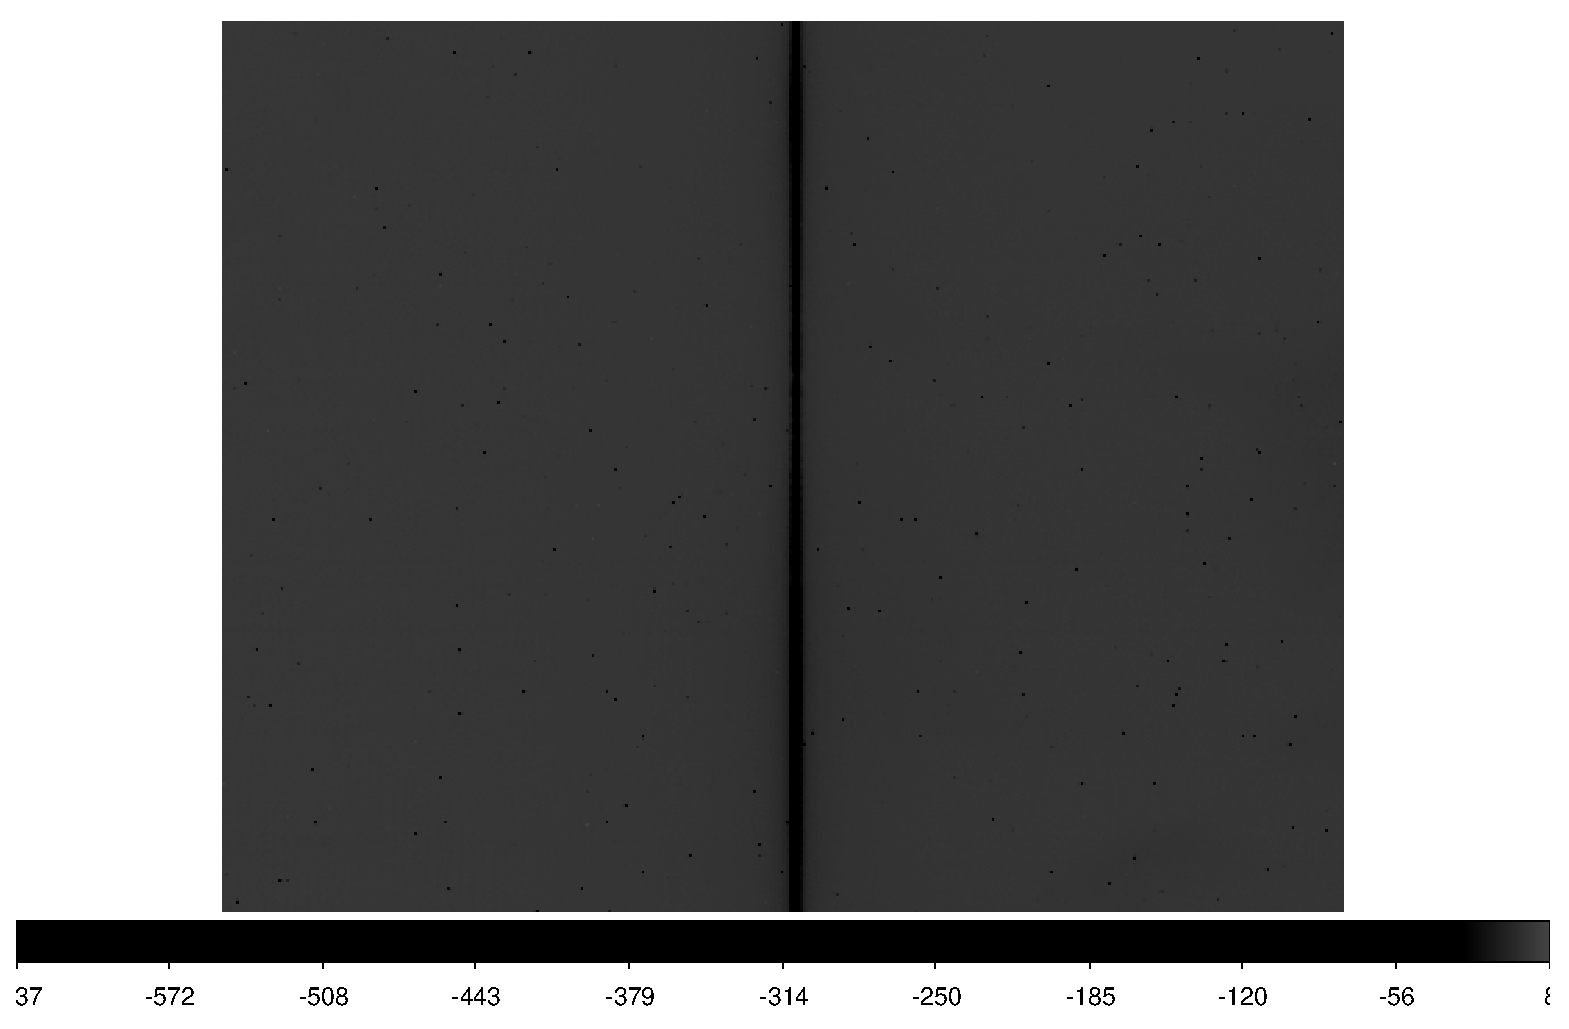
\includegraphics[width=0.645\linewidth]{SLIT7_Y} \\ фильтр YOS}
\end{minipage}
\begin{minipage}[h]{0.50\linewidth}
\center{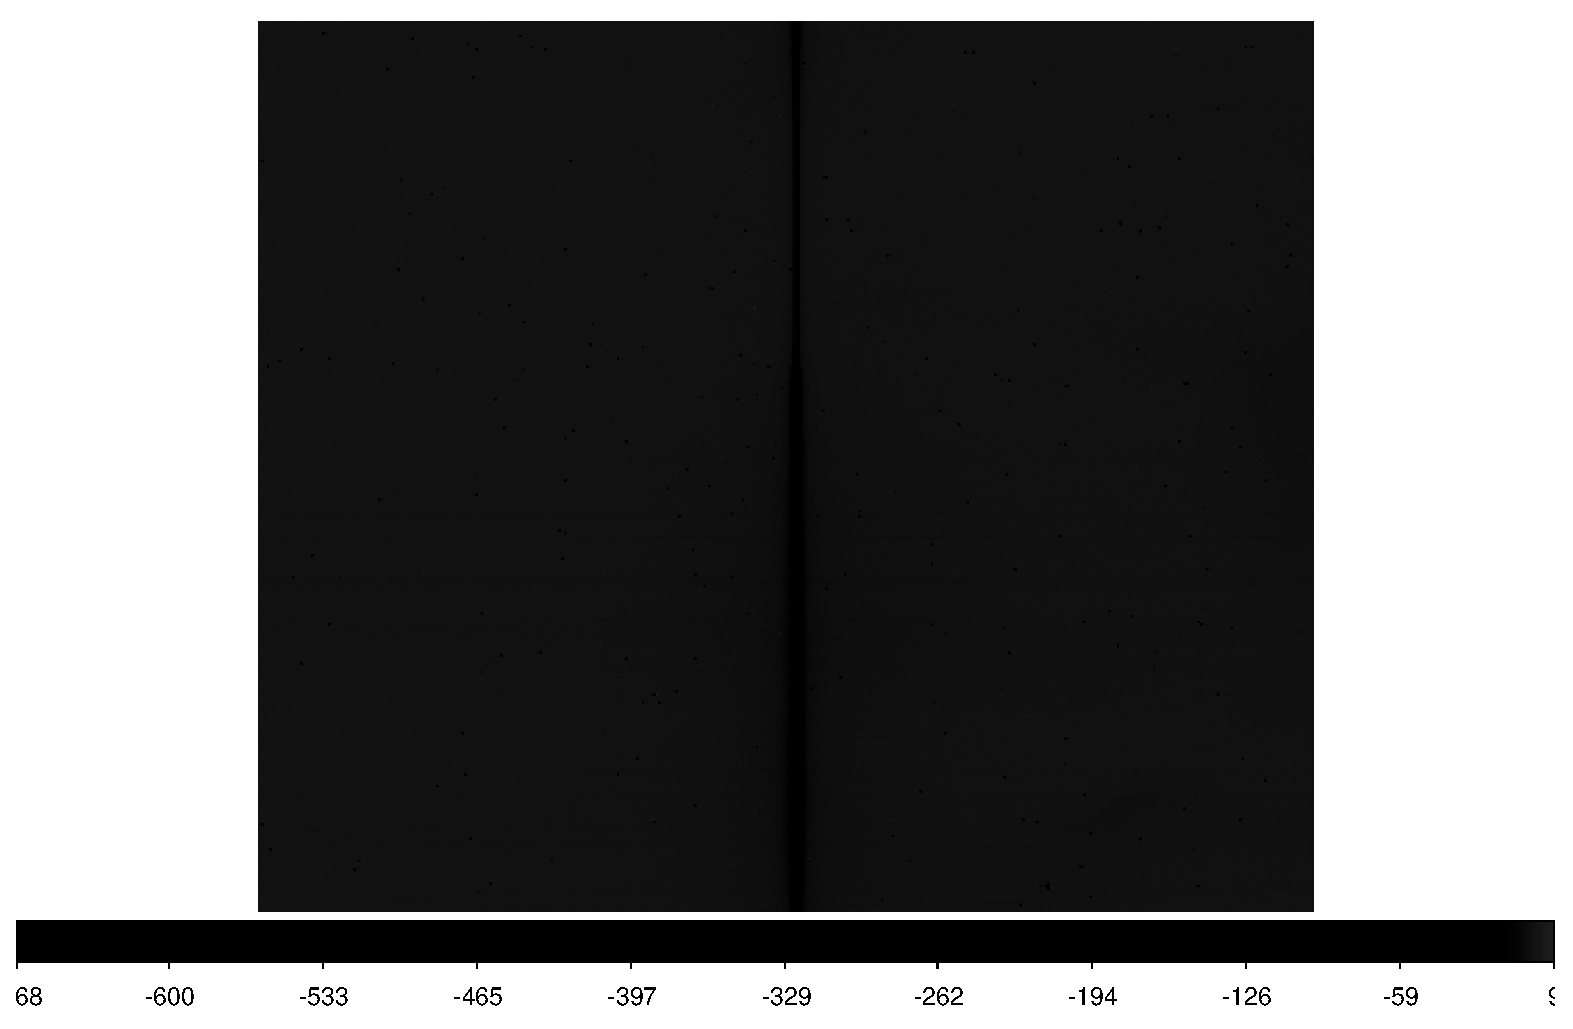
\includegraphics[width=0.64\linewidth]{SLIT7_J} \\ фильтр JOS}
\end{minipage}
\begin{minipage}[h]{0.50\linewidth}
\center{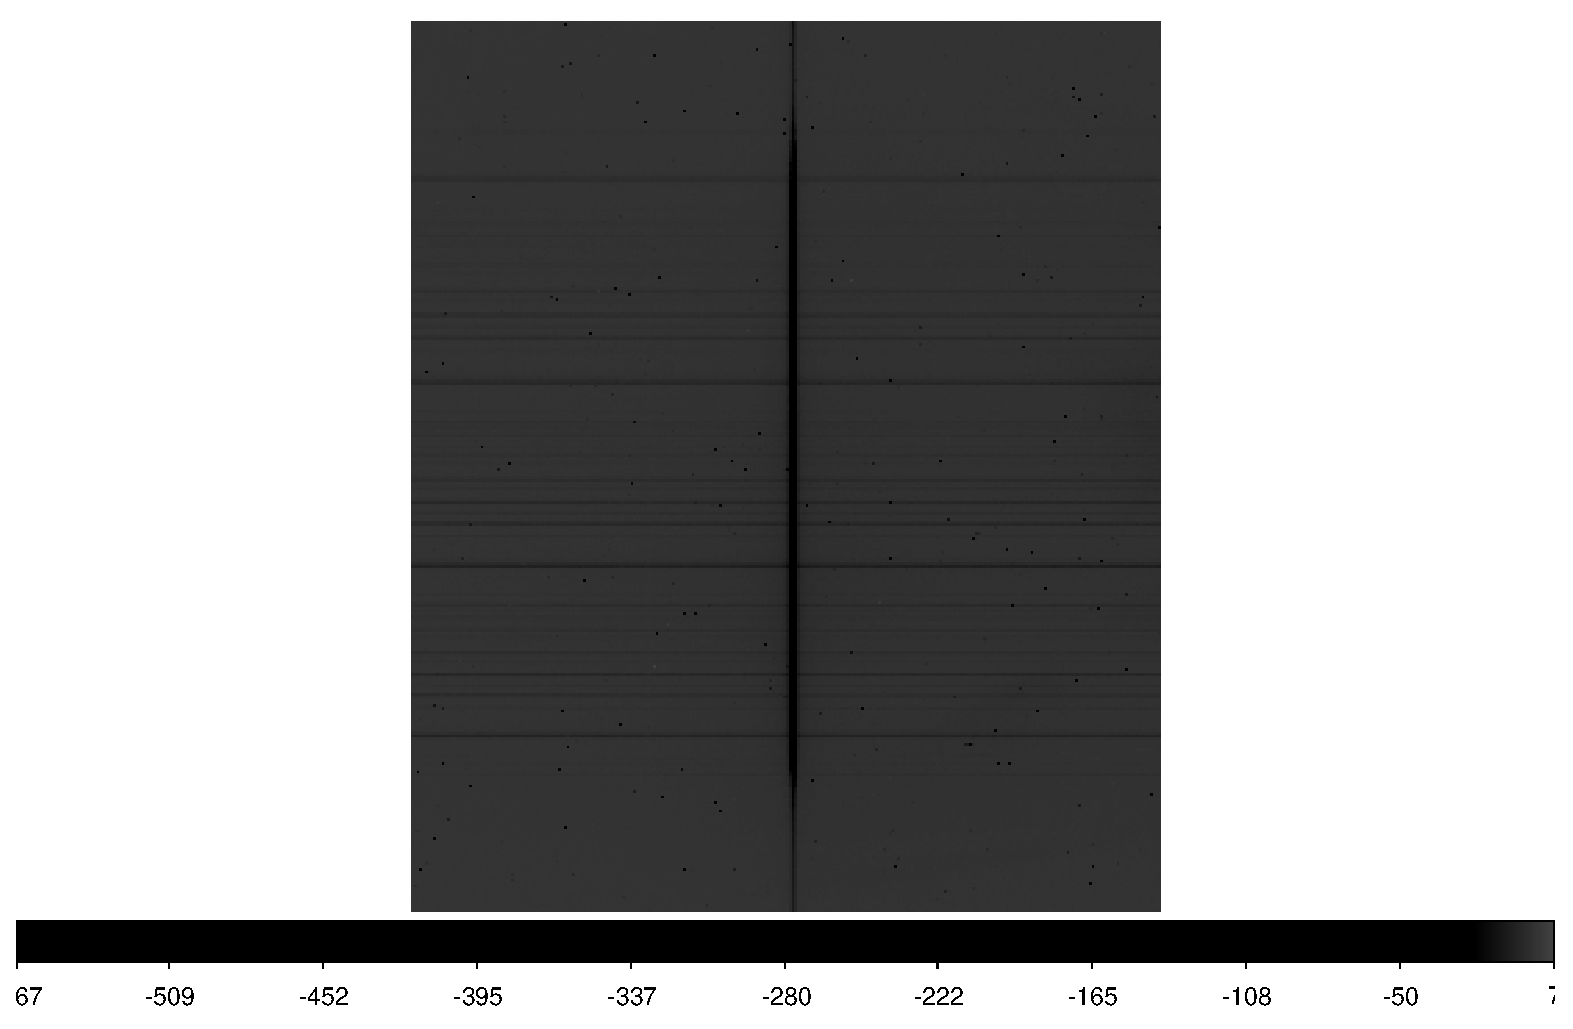
\includegraphics[width=0.64\linewidth]{SLIT7_H} \\ фильтр H}
\end{minipage}
\begin{minipage}[h]{0.50\linewidth}
\center{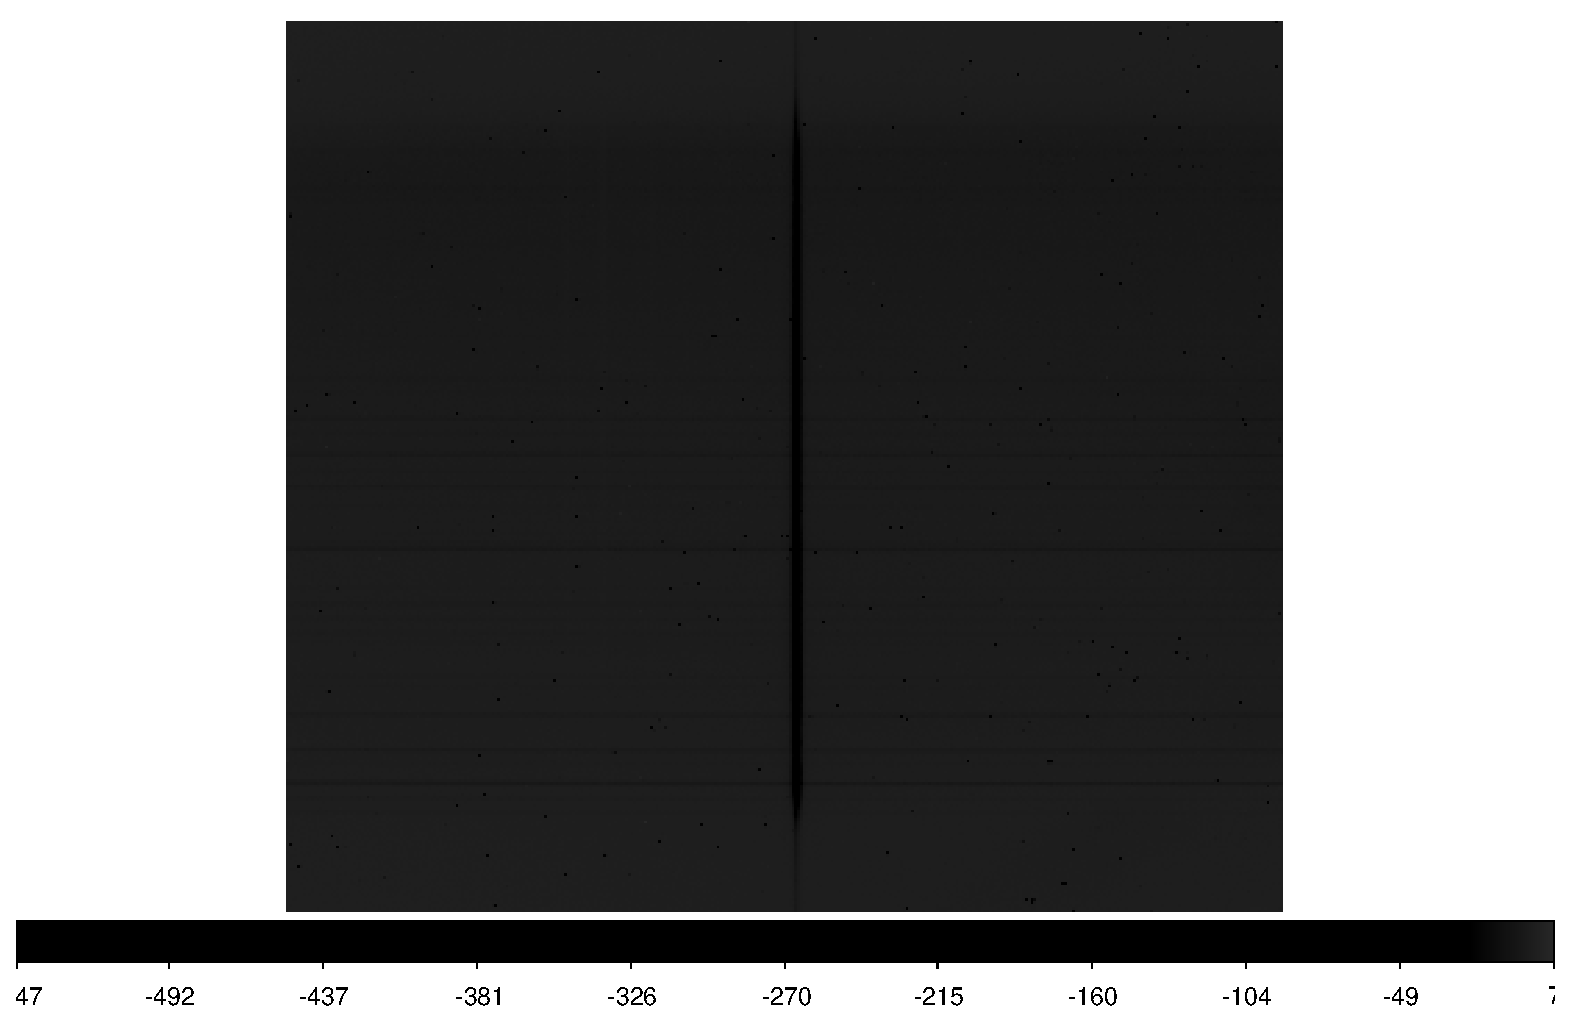
\includegraphics[width=0.64\linewidth]{SLIT7_K} \\ фильтр K}
\end{minipage}
\caption{Спектры звезды с использованием спектральной щели SLIT7 (с атмосферными полосами).}
\label{ris:image2}
\end{figure}

Наличие атмосферных полос на спектрах, полученных с использованием спектральной щели SLIT7, объясняется наличием рассеянного в атмосфере света. Как можно заметить, данные полосы в первом приближении прямые и можно пренебречь их кривизной. Следовательно, путём несложных операций по вычитанию от них можно избавиться. И в результате были получены изображения, представленные на Рис. 4.

\begin{figure}[h]
\begin{minipage}[h]{0.50\linewidth}
\center{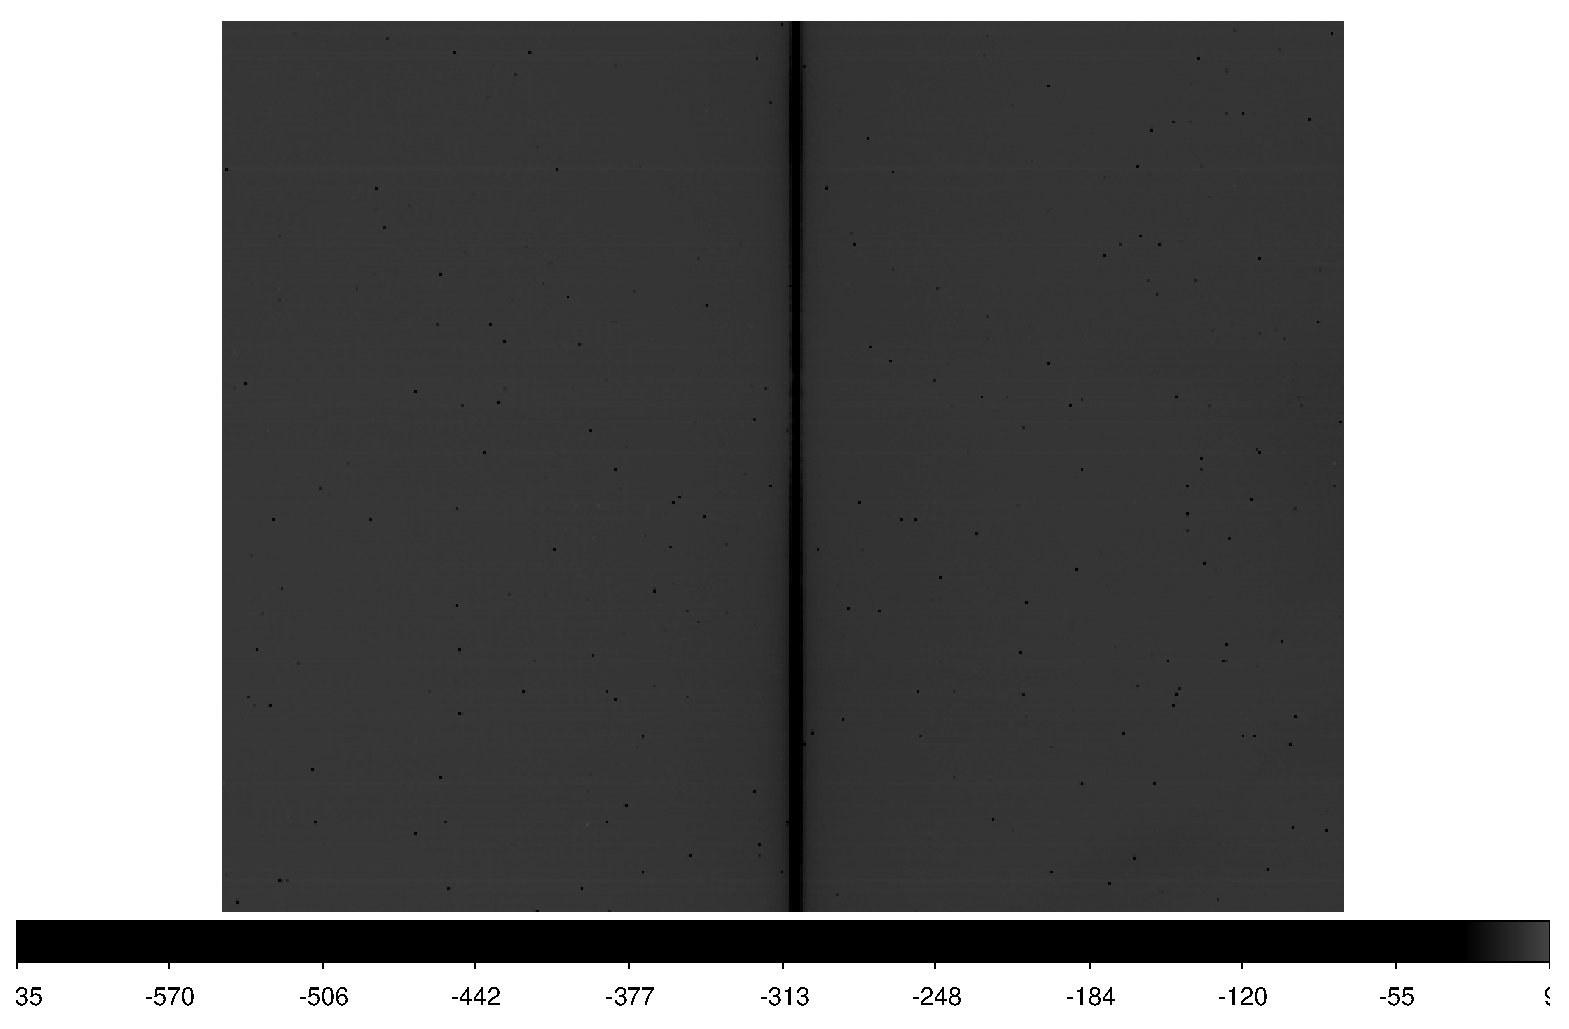
\includegraphics[width=0.64\linewidth]{SLIT7_Yw} \\ фильтр YOS}
\end{minipage}
\begin{minipage}[h]{0.50\linewidth}
\center{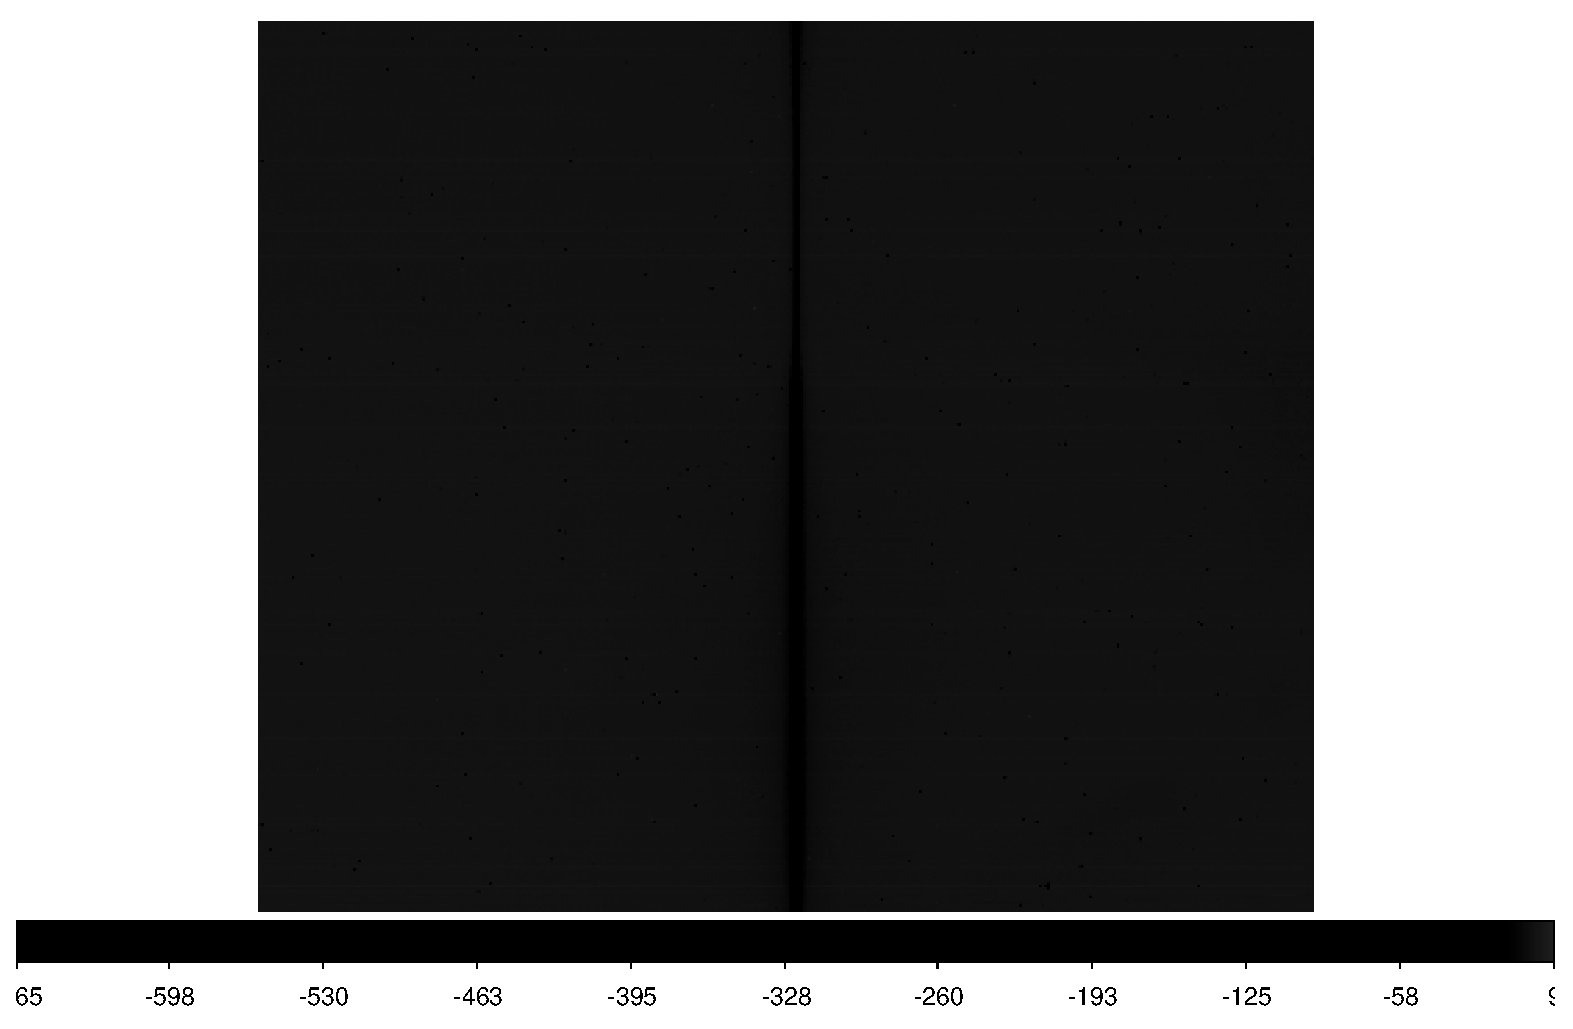
\includegraphics[width=0.64\linewidth]{SLIT7_Jw} \\ фильтр JOS}
\end{minipage}
\begin{minipage}[h]{0.50\linewidth}
\center{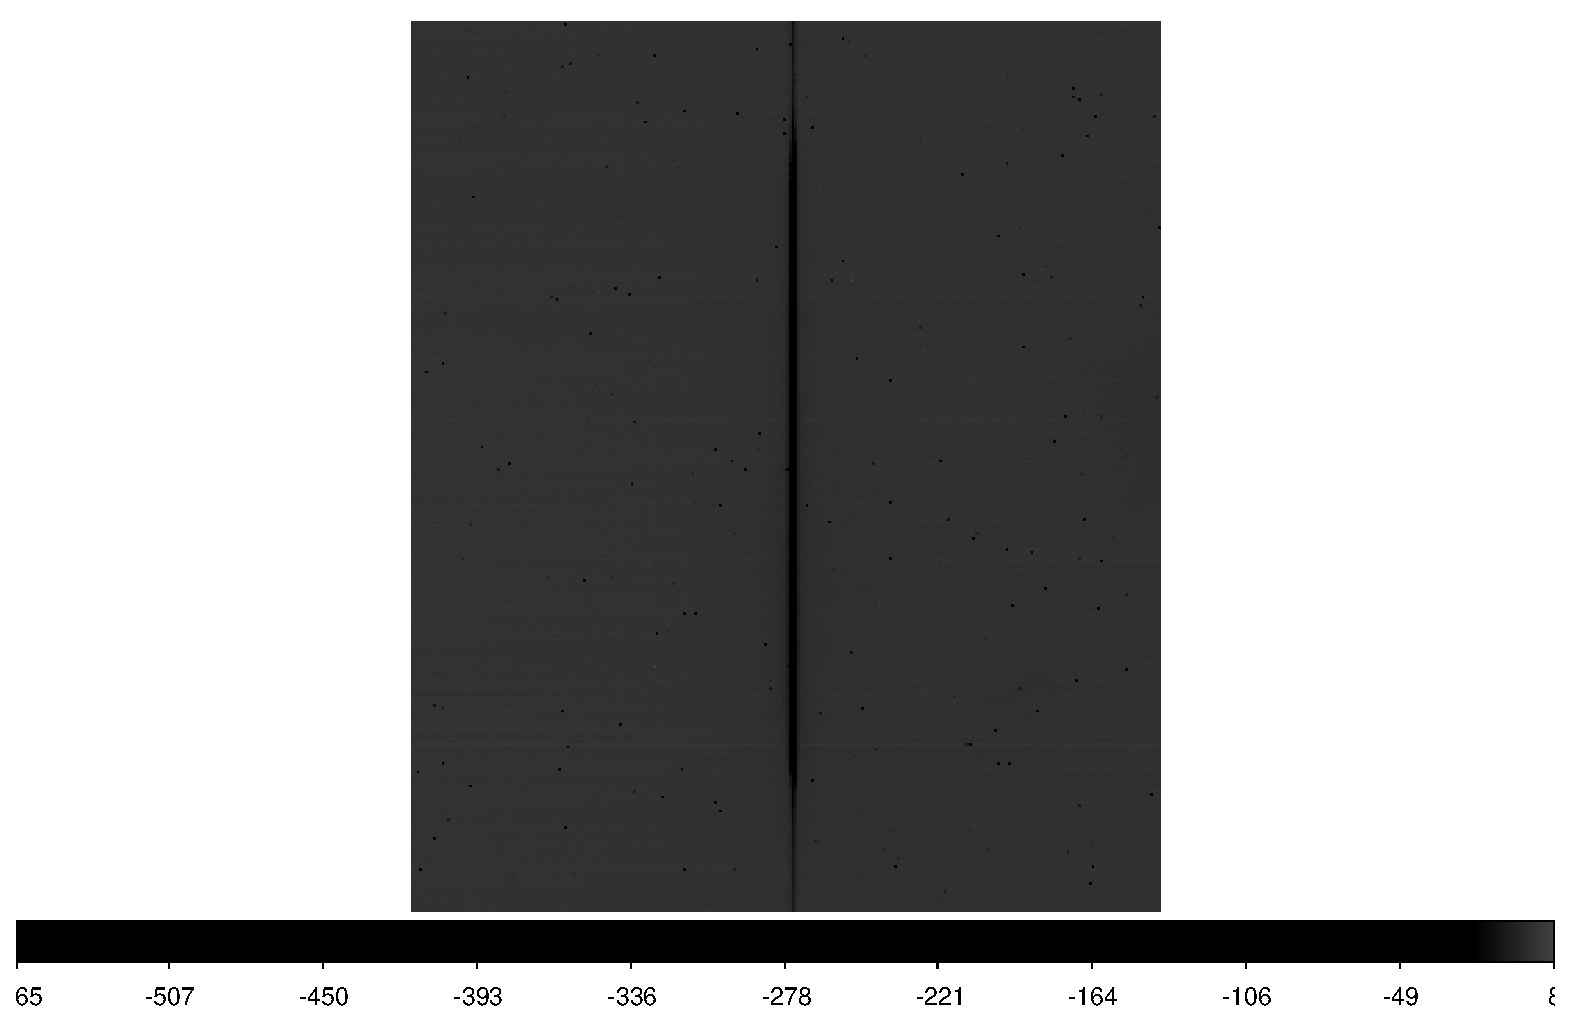
\includegraphics[width=0.64\linewidth]{SLIT7_Hw} \\ фильтр H}
\end{minipage}
\begin{minipage}[h]{0.50\linewidth}
\center{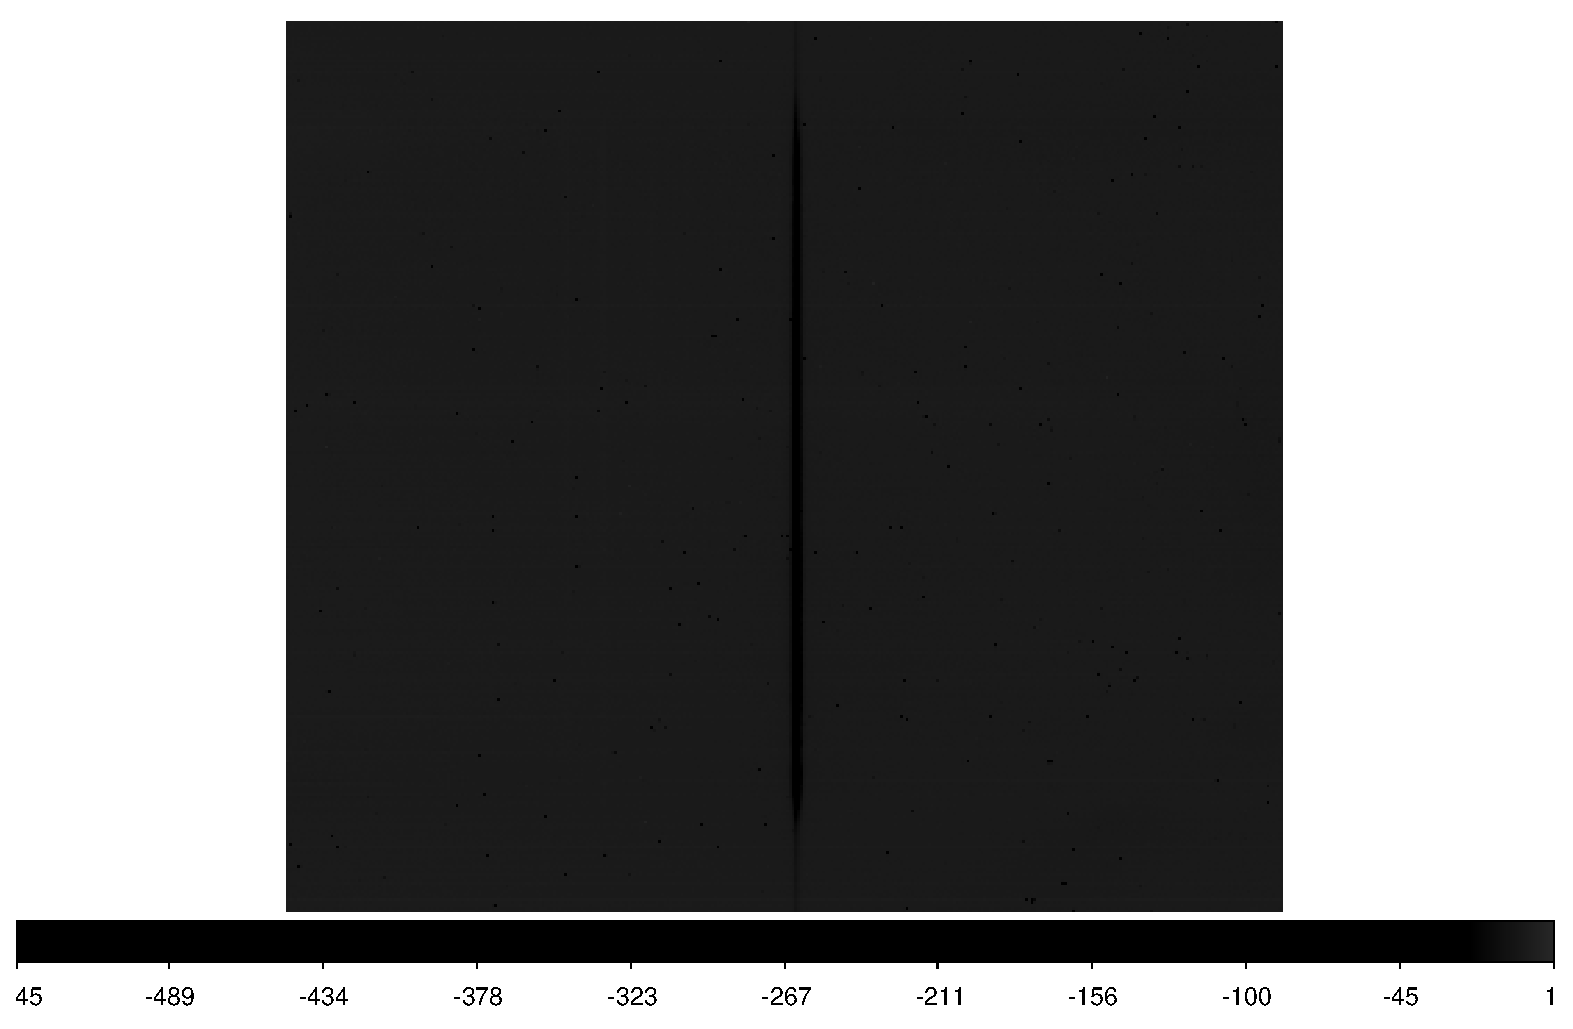
\includegraphics[width=0.64\linewidth]{SLIT7_Kw} \\ фильтр K}
\end{minipage}
\caption{Спектры звезды с использованием спектральной щели SLIT7 (без атмосферных полос).}
\label{ris:image3}
\end{figure}

\hfill\break
Полученые в результате обработки фотографий спектры мы использовали для нахождения величины эффективности системы "атмосфера+телескоп+камера".
\section{Обработка данных}
Для обработки данных был необходим стандарт спектра звезды спектрального класса A0V, чтобы сравнить с данным эталоном вне атмосферы наши экспериментально полученные данные. В качестве такого был взят спектр звезды $\alpha Lyr$ (Вега) из источника \cite{Vega}. Данный спектр был дан в относительных единицах, но, зная потоки Веги в различных фильтрах и кривые пропускания фильтров, можно получить поток от Веги в $\frac{\text{эрг}}{\text{см}^2\cdot\text{с}\cdot\text{см}}$:
\begin{eqnarray*}
E_{Y} =  5.81\cdot10^{-2} \frac{\text{эрг}}{\text{см}^2\cdot\text{с}\cdot\text{см}},\\
E_{J} =  3.14\cdot10^{-2} \frac{\text{эрг}}{\text{см}^2\cdot\text{с}\cdot\text{см}},\\
E_{H} =  1.20\cdot10^{-2} \frac{\text{эрг}}{\text{см}^2\cdot\text{с}\cdot\text{см}},\\
E_{K} =  0.412\cdot10^{-2} \frac{\text{эрг}}{\text{см}^2\cdot\text{с}\cdot\text{см}}.\\
\end{eqnarray*}

Также необходимо было учесть время выдержки изображения $\tau$ и, что площадь главного зеркала телескопа рассчитывается по формуле: $S_{mirror} = \pi\cdot\frac{d^2}{4}$, где $\pi\approx 3.14, d = 2.5 \text{м}$ - диаметр главного зеркала телескопа. Учитывая это и нормируя на величину $h\nu_i$, мы получим спектр звезды $\alpha Lyr$ в $\frac{\text{Nph}}{\Delta\lambda}$, т.е. мы получили для звезды $\alpha Lyr$ зависимость числа фотонов, падающих на границу атмосферы площадью $S_{mirror}$, за время выдержки $\tau$, в единичном спектральном интервале длин волн $\Delta\lambda$ в зависимости от длины волны. Звёздная величина звезды HIP85382 в различных фильтрах:
\begin{eqnarray*}
m_Y = 5.924\pm 0,025; \\
m_J = 5.901\pm 0.034; \\
m_H = 5.955\pm 0.023; \\
m_K = 5.915\pm 0.017;
\end{eqnarray*}

Используя формулу Погсона для Веги и звезды HIP85382: $m_{HIP85382_i} - m_{\alpha Lyr_i}= -2,5lg{\frac{E_{HIP85382_i}}{E_{\alpha Lyr_i}}}$ и зная звёздные величины звезды HIP85382 в интерисующих нас фильтрах, был найден коэффициент, связывающий имеющийся у нас спектр для Веги и спектр звезды HIP85382. Для звезды HIP85382 был получен график, изображённый на Рис. 5\footnote{На самом деле звёздные величины для звезды спектрального класса A0 одинаковы для всех фильтров с точностью до ошибки поэтому достаточно использовать какой-либо один фильтр при вычислении нормировочной постоянной и перевода спектра Веги в спектр для нашей звезды.}.

Домножая спектр Веги на постоянную величину и делая свёртку получившегося спектра с кривыми фильтра Y,J,H,K, был получен инетерсующий нас спектр исследуемой звезды  (HIP85382) в соответствующих фильтрах, в единицах $\frac{Nph}{\Delta\lambda}$. Эти полученные зависимости мы использовали для дальнейшего сравнения с нашими экспериментальными данными.
%Чому для разных фильтров спектры веги разные, нормировочные постоянные
\begin{figure}[h]
\center{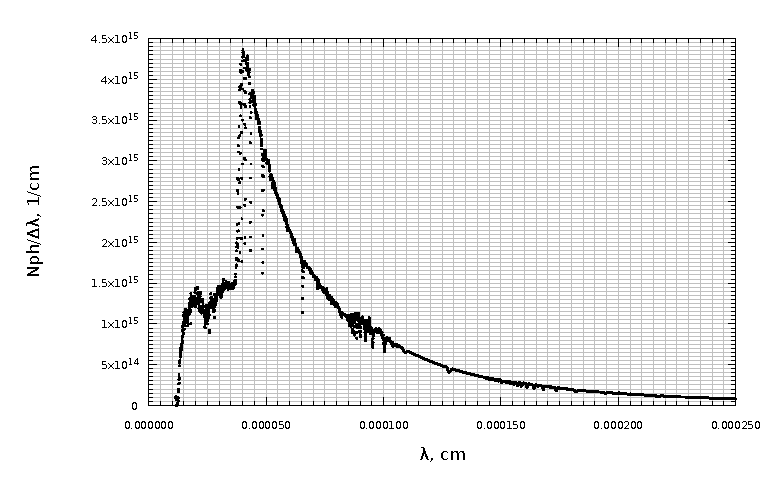
\includegraphics[width=0.85\linewidth]{our_star_phot}}
\caption{Число фотонов, падающих на границу атмосферы площадью $S_{mirror}$, за время выдержки $\tau$, в единичном спектральном интервале длин волн $\Delta\lambda$, для звезды HIP85382.}
\label{ris:image}
\end{figure}

Из полученных изображений спектра также несложно было получить такие же зависимости $\frac{Nph}{\Delta\lambda}$ в зависимости от длины волны, используя дисперсионные кривые. Заметим, что у получившихся спектров в фильтрах Y и J существуют заметные полосы поглощения, происхождение которых можно объяснить линиями поглощения молекулами водяного пара в атмосфере \cite{vapour}. Соответственно, можно было интерполировать данные из нашего стандарта на экспериментальные данные и, разделив их, мы смогли численно оценить значения коэффициента пропускания системы "атмосфера+телескоп+камера". В приложении можно найти графики зависимостей коэффициента эффективности для каждого фильтра и разных щелей в отдельности. Пилообразная форма объясняется наличием экстинкции атмосферы. Стоит также отметить, что обработка изображений в большей степени зависела от числа выбранных пикселей, которые в дальнейшем и стали представлять собой наш полученный спектр. На данных графиках была сделана выборка в 30 пикселей. Данный эффект можно объяснить тем, что имеющиеся спектры были испорчены влиянием атмосферы, которая была сверхвлажная в дни съёмки, а также не стоит пренебрегать тем эффектом, что исследуемая звезда

%\begin{figure}[h]
%\center{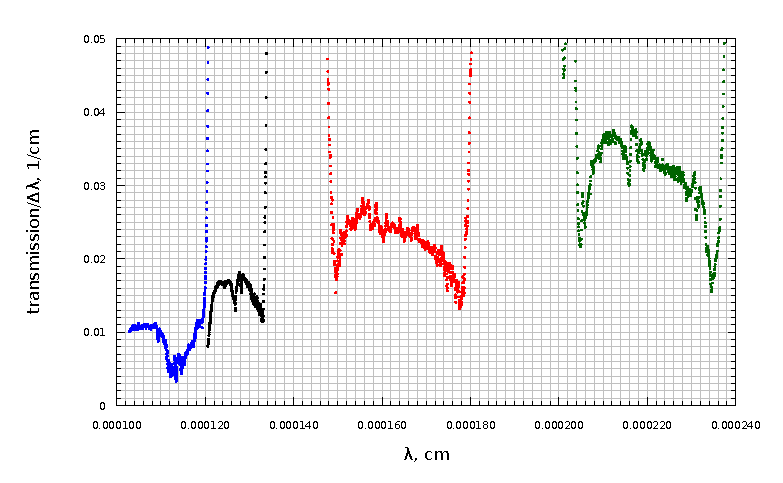
\includegraphics[width=0.8\linewidth]{../handle/SLIT6/all_in_res} \\ SLIT6}
%\end{figure}
%\begin{figure}[h]
%\center{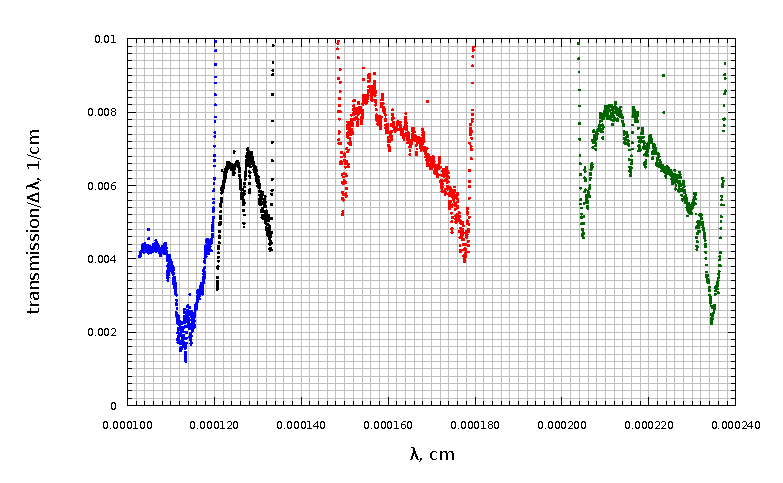
\includegraphics[width=0.8\linewidth]{../handle/SLIT7/all_in_res} \\ SLIT7}
%\end{figure}

\noindent находилась относительно на небольшой высоте. Как следствие мы получили тот факт, что оценка средней величины эффективности была осложнена и варьировалась, помимо этого присутствовали ошибки при интерполяции графиков. Однако, в данной работе можно было ограничиться верхней численной оценкой для каждого из фильтров и соответсвующей ей спектральной щели.

\hfill\break

\section{Итог}
В результате обработки спектров были получены зависимости величины эффективности (или пропускания) системы "атмосфера+телескоп+камера", приходящейся на единичный интервал длин волн, в зависимости от длины волны для различных фильтров YOS, JOS, H, K, и для спектральных щелей SLIT6 и SLIT7 соответсвенно. Эти данные можно посмотреть в Приложении.

\newpage
\section{Приложения}

\begin{figure}[h]
\center{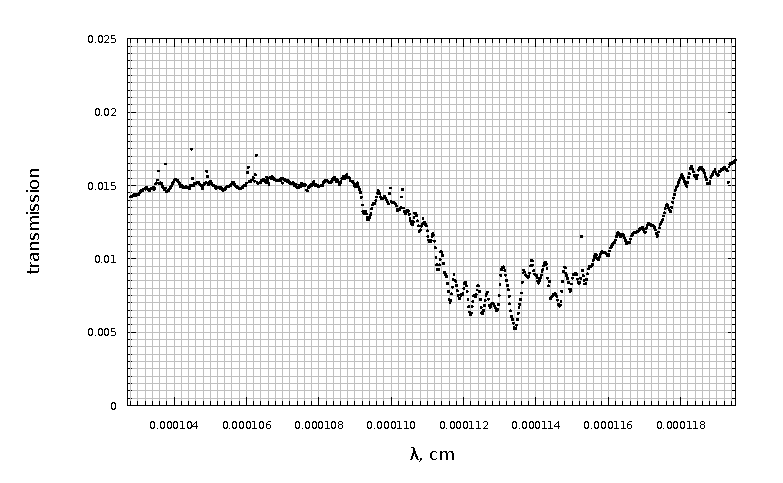
\includegraphics[width=0.8\linewidth]{../handle/SLIT6/interpolated_teor_to_pracY} \\ График зависимости пропускания от длины волны для спектральной щели SLIT6 (фильтр Y).}
\end{figure}
\begin{figure}[h]
\center{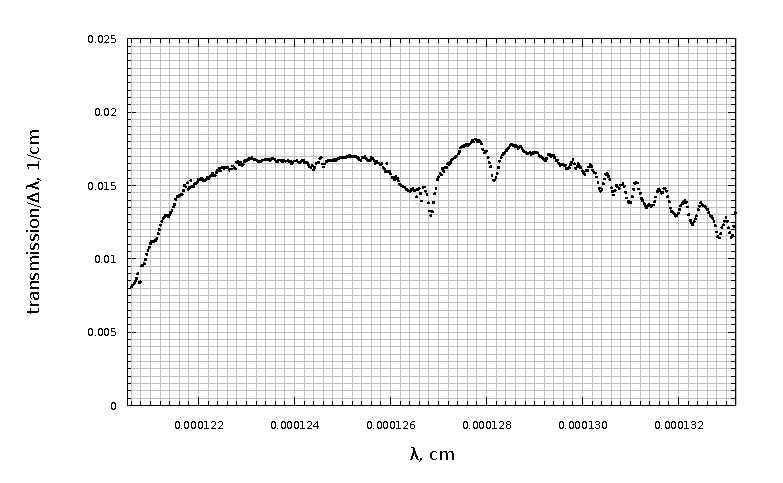
\includegraphics[width=0.8\linewidth]{../handle/SLIT6/interpolated_teor_to_pracJ} \\  График зависимости пропускания от длины волны для спектральной щели SLIT6 (фильтр J).}
\end{figure}
\begin{figure}[h]
\center{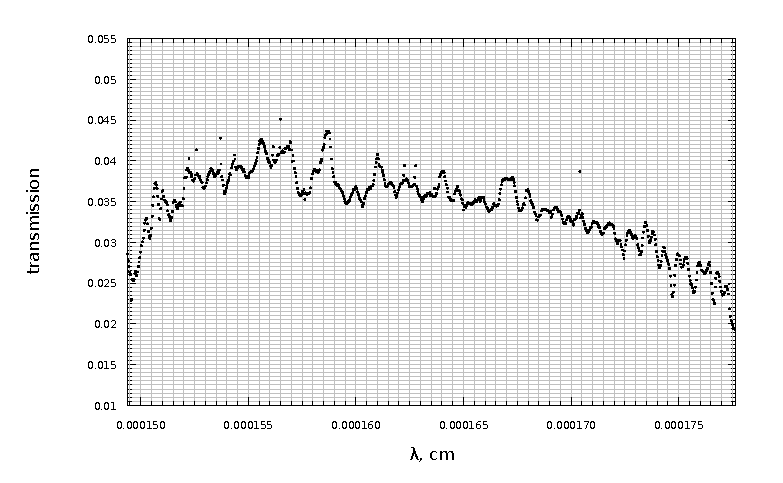
\includegraphics[width=0.8\linewidth]{../handle/SLIT6/interpolated_teor_to_pracH} \\ График зависимости пропускания от длины волны для спектральной щели SLIT6 (фильтр H.)}
\end{figure}
\begin{figure}[h]
\center{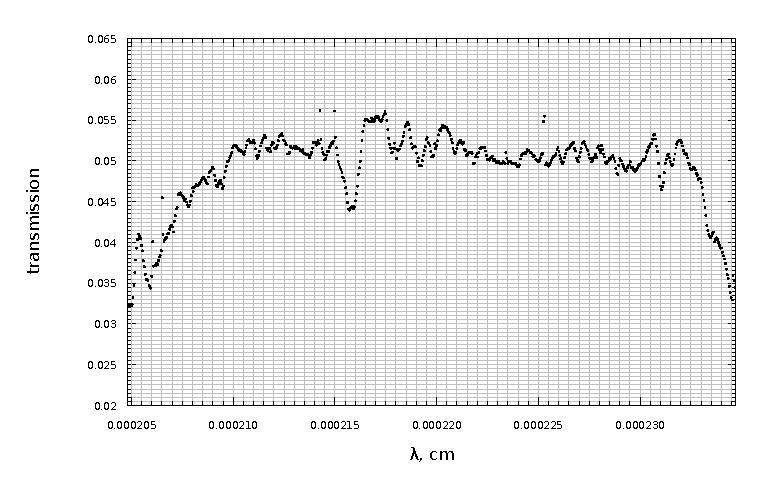
\includegraphics[width=0.8\linewidth]{../handle/SLIT6/interpolated_teor_to_pracK} \\  График зависимости пропускания от длины волны для спектральной щели SLIT6 (фильтр K).}
\end{figure}
\begin{figure}[h]
\center{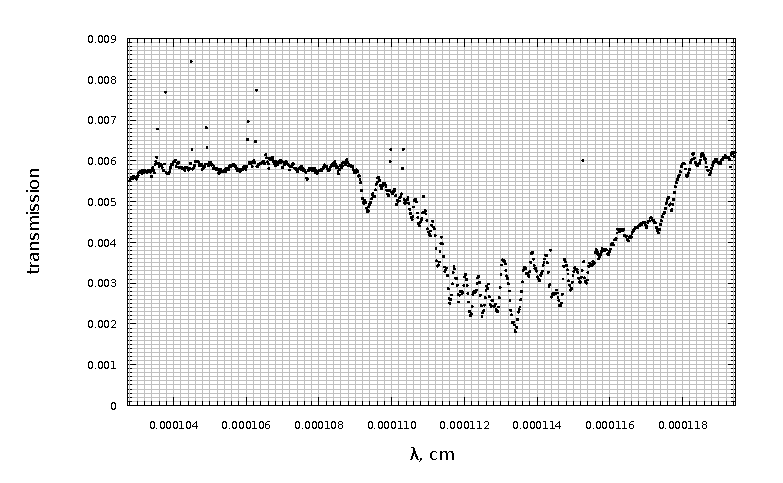
\includegraphics[width=0.8\linewidth]{../handle/SLIT7/interpolated_teor_to_pracY} \\  График зависимости пропускания от длины волны для спектральной щели SLIT7 (фильтр Y).}
\end{figure}
\begin{figure}[h]
\center{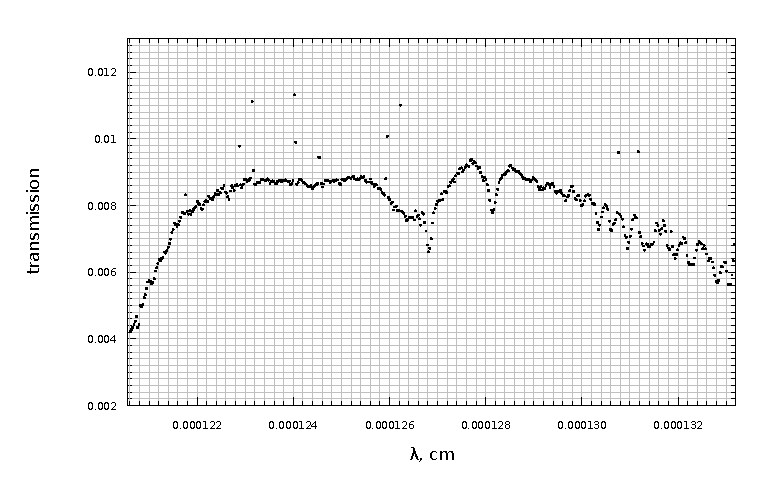
\includegraphics[width=0.8\linewidth]{../handle/SLIT7/interpolated_teor_to_pracJ} \\  График зависимости пропускания от длины волны для спектральной щели SLIT7 (фильтр J).}
\end{figure}
\begin{figure}[h]
\center{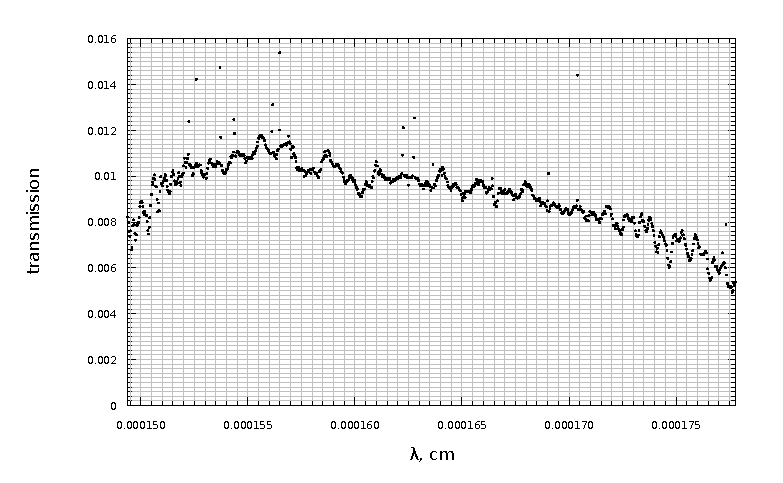
\includegraphics[width=0.8\linewidth]{../handle/SLIT7/interpolated_teor_to_pracH} \\  График зависимости пропускания от длины волны для спектральной щели SLIT7 (фильтр H).}
\end{figure}
\begin{figure}[h]
\center{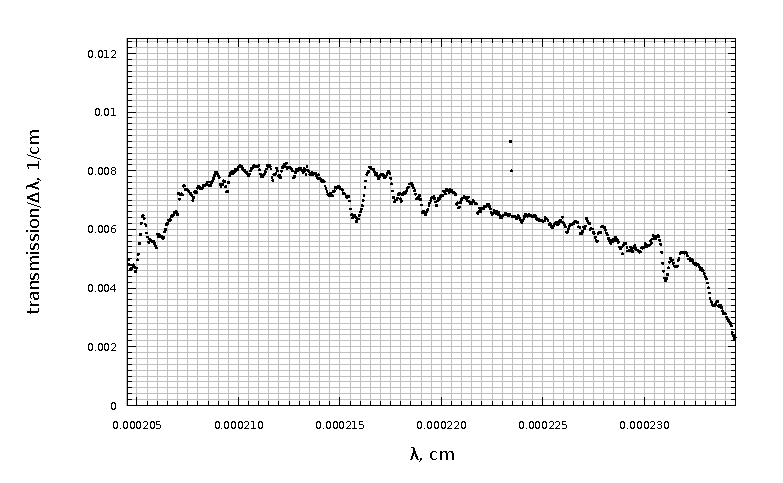
\includegraphics[width=0.8\linewidth]{../handle/SLIT7/interpolated_teor_to_pracK} \\  График зависимости пропускания от длины волны для спектральной щели SLIT7 (фильтр K).}
\end{figure}
\begin{figure}[h]
\begin{minipage}[h]{0.5\linewidth}
\center{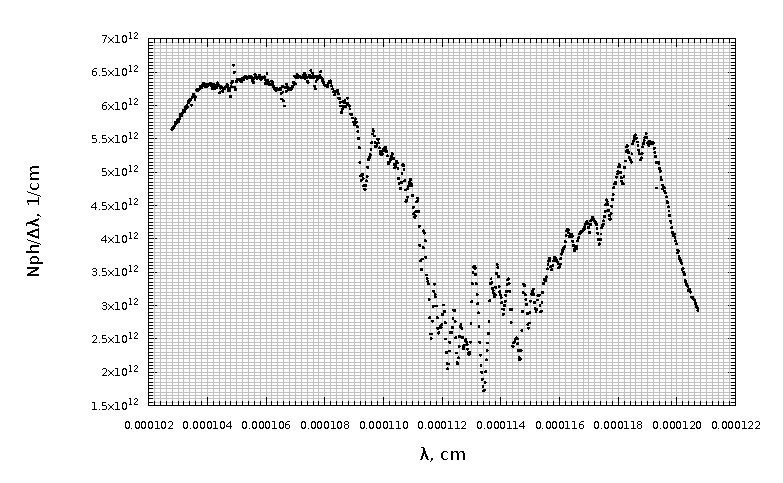
\includegraphics[width=1\linewidth]{n_hip85382-YOS-G-20180710232047-85_linearYcorr_spectr_abs} \\ фильтр Y (эксперимент)}
\end{minipage}
\begin{minipage}[h]{0.5\linewidth}
\center{\includegraphics[width=1\linewidth]{../handle/SLIT6/our_star_photY} \\ фильтр Y (теория)}
\end{minipage}
\begin{minipage}[h]{0.5\linewidth}
\center{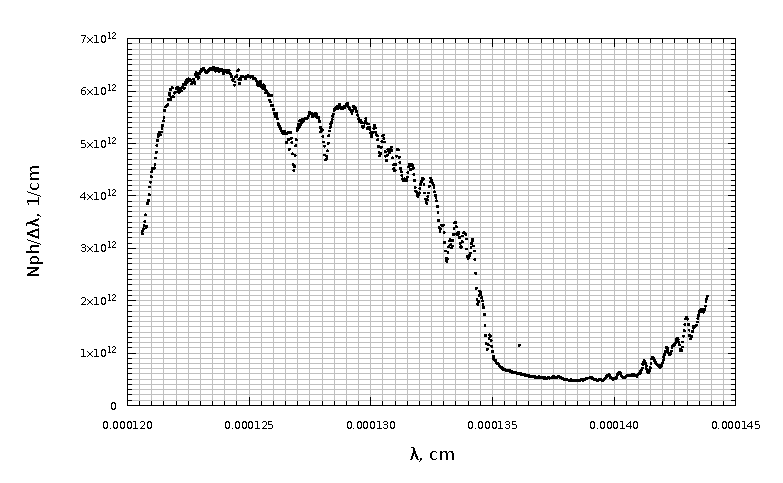
\includegraphics[width=1\linewidth]{n_hip85382-JOS-G-20180710232307-86_linearYcorr_spectr_abs} \\ фильтр J (эксперимент)}
\end{minipage}
\begin{minipage}[h]{0.5\linewidth}
\center{\includegraphics[width=1\linewidth]{../handle/SLIT6/our_star_photJ} \\ фильтр J (теория)}
\end{minipage}
\begin{minipage}[h]{0.5\linewidth}
\center{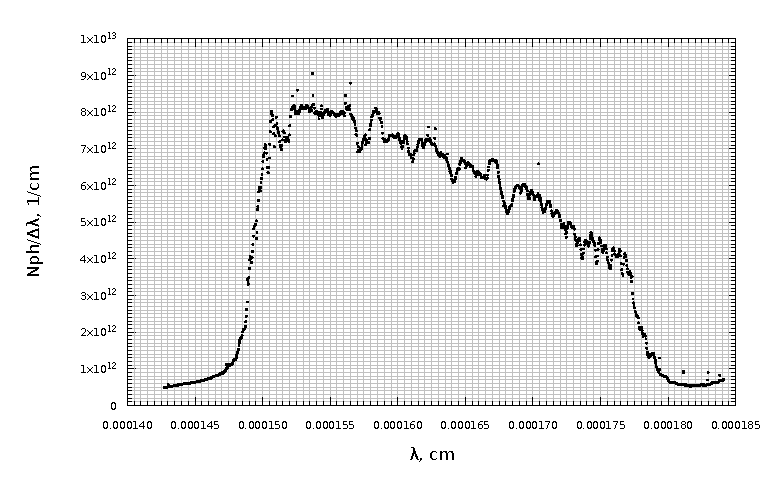
\includegraphics[width=1\linewidth]{n_hip85382-H-G-20180710232600-87_linearYcorr_spectr_abs} \\ фильтр H (теория)}
\end{minipage}
\begin{minipage}[h]{0.5\linewidth}
\center{\includegraphics[width=1\linewidth]{../handle/SLIT6/our_star_photH} \\ фильтр H (теория)}
\end{minipage}
\begin{minipage}[h]{0.5\linewidth}
\center{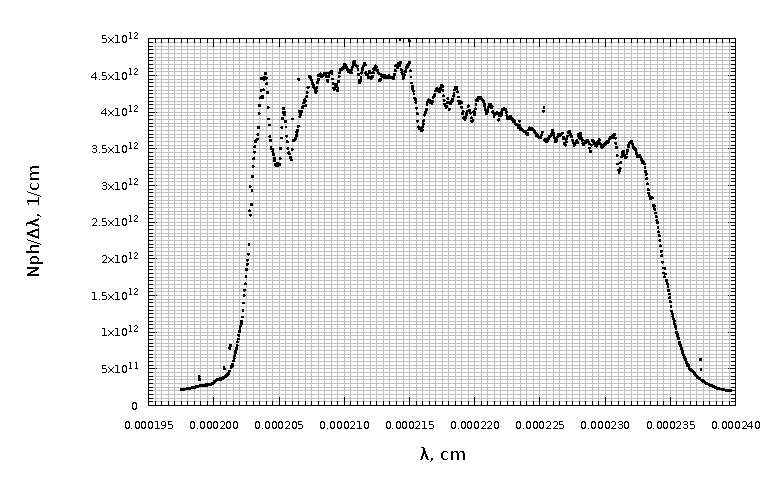
\includegraphics[width=1\linewidth]{n_hip85382-K-G-20180710232812-88_linearYcorr_spectr_abs} \\ фильтр K (эксперимент)}
\end{minipage}
\begin{minipage}[h]{0.5\linewidth}
\center{\includegraphics[width=1\linewidth]{../handle/SLIT6/our_star_photK} \\ фильтр K (теория)}
\end{minipage}
\caption{Графики зависимостей числа фотонов в полосе $\Delta\lambda$ от длины волны для спектральной щели SLIT6.}
\end{figure}

\begin{figure}[h]
\begin{minipage}[h]{0.5\linewidth}
\center{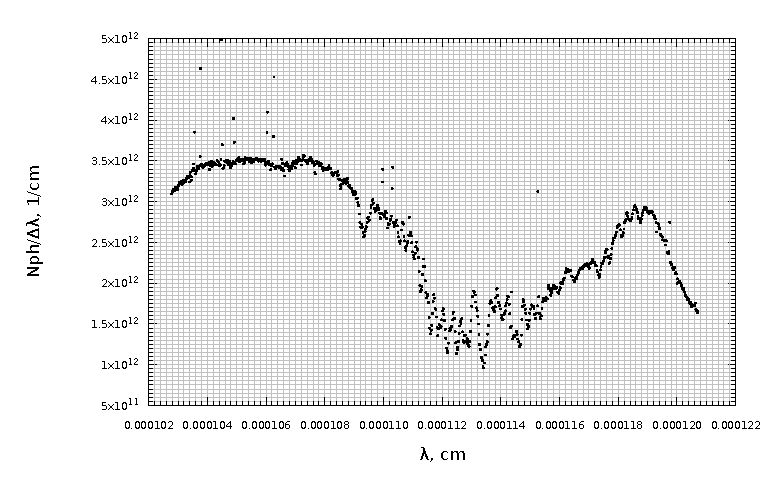
\includegraphics[width=1\linewidth]{y_hip85382-YOS-G-20180710233220-89_linearYcorr_spectr_abs} \\ фильтр Y (эксперимент)}
\end{minipage}
\begin{minipage}[h]{0.5\linewidth}
\center{\includegraphics[width=1\linewidth]{../handle/SLIT7/our_star_photY} \\ фильтр Y (теория)}
\end{minipage}
\begin{minipage}[h]{0.5\linewidth}
\center{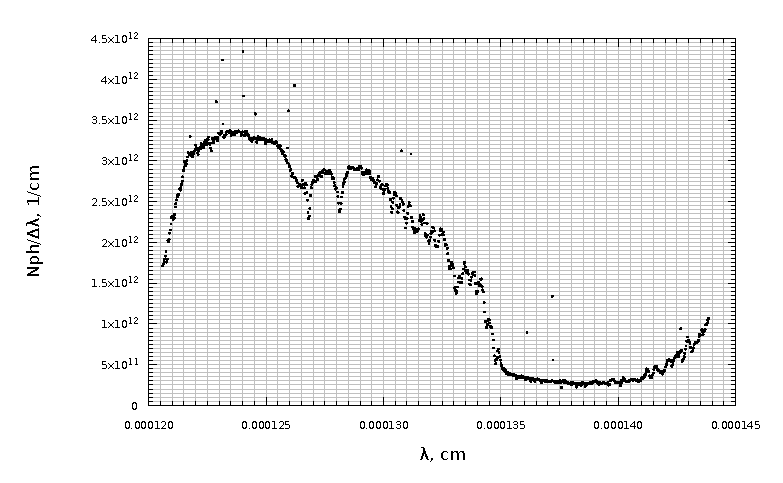
\includegraphics[width=1\linewidth]{y_hip85382-JOS-G-20180710233424-90_linearYcorr_spectr_abs} \\ фильтр J (эксперимент)}
\end{minipage}
\begin{minipage}[h]{0.5\linewidth}
\center{\includegraphics[width=1\linewidth]{../handle/SLIT7/our_star_photJ} \\ фильтр J (теория)}
\end{minipage}
\begin{minipage}[h]{0.5\linewidth}
\center{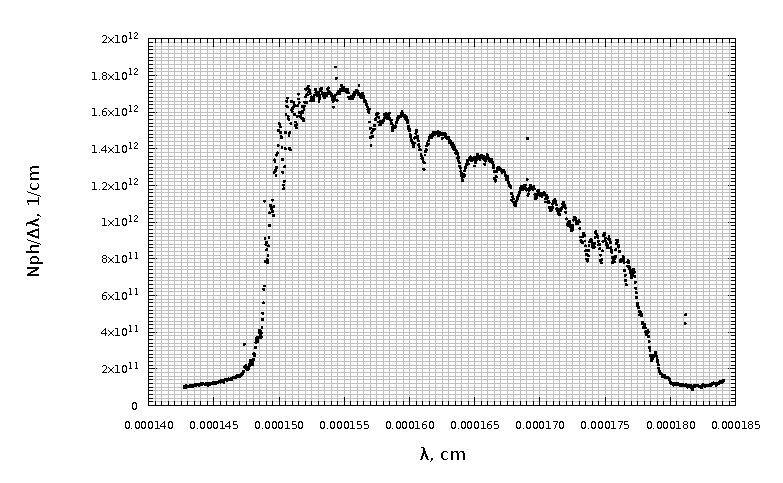
\includegraphics[width=1\linewidth]{y_hip85382-H-G-20180710233655-91_linearYcorr_spectr_abs} \\ фильтр H (теория)}
\end{minipage}
\begin{minipage}[h]{0.5\linewidth}
\center{\includegraphics[width=1\linewidth]{../handle/SLIT7/our_star_photH} \\ фильтр H (теория)}
\end{minipage}
\begin{minipage}[h]{0.5\linewidth}
\center{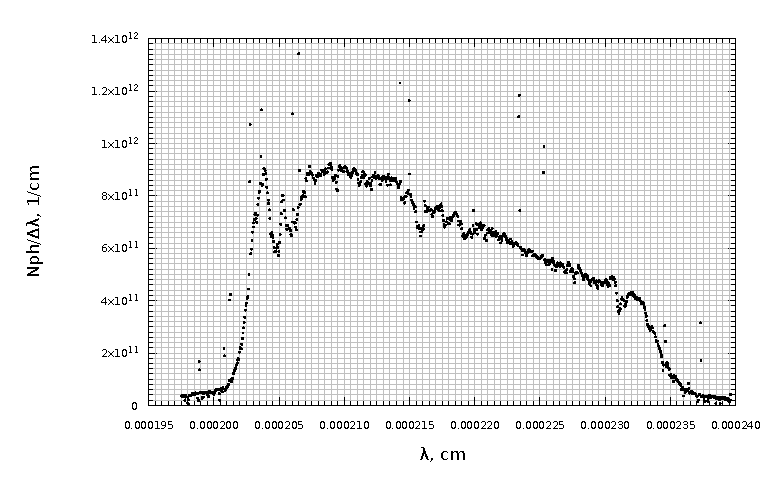
\includegraphics[width=1\linewidth]{y_hip85382-K-G-20180710233908-92_linearYcorr_spectr_abs} \\ фильтр K (эксперимент)}
\end{minipage}
\begin{minipage}[h]{0.5\linewidth}
\center{\includegraphics[width=1\linewidth]{../handle/SLIT7/our_star_photK} \\ фильтр K (теория)}
\end{minipage}
\caption{Графики зависимостей числа фотонов в полосе $\Delta\lambda$ от длины волны для спектральной щели SLIT7.}
\end{figure}
\clearpage

\begin{figure}[h]
\center{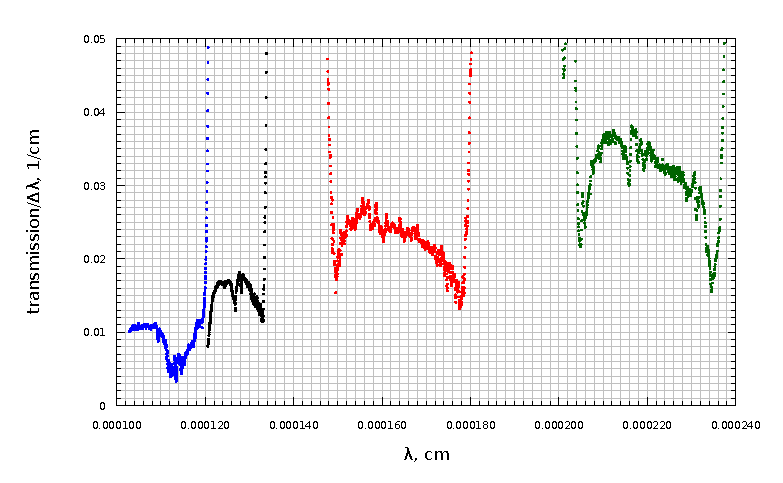
\includegraphics[width=0.77\linewidth]{../handle/SLIT6/all_in_res} \\ График зависимостей пропусканий от длины волны для четырёх фильтров при использовании спектральной щели SLIT6.}
\end{figure}
\begin{figure}[h]
\center{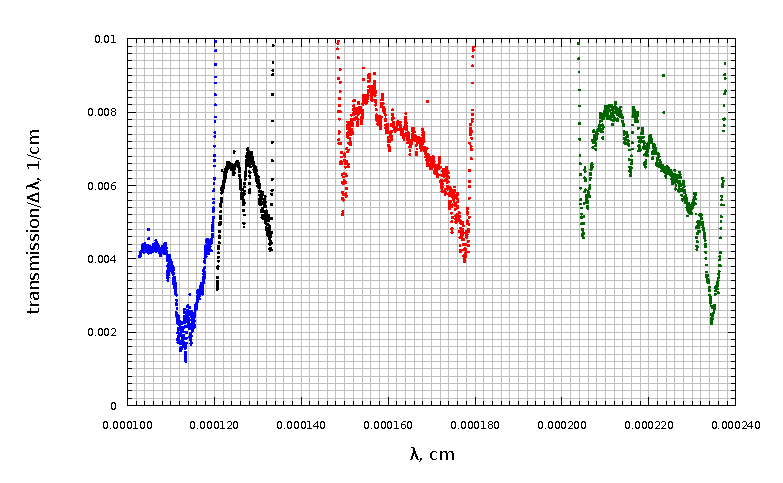
\includegraphics[width=0.77\linewidth]{../handle/SLIT7/all_in_res} \\ График зависимостей пропусканий от длины волны для четырёх фильтров при использовании спектральной щели SLIT7.}
\end{figure}

\hfill\break
\newpage
\begin{thebibliography}{3}
\bibitem{Sulsky1994}
А. Э. Наджип, А. М. Татарников, Д. У. Туми, Н. И. Шатский, А. М. Черепащук, С. А. Ламзин, А. А. Белинский,  ASTRONIRCAM - инфракрасная камера-спектрограф 2.5-м телескопа КГО ГАИШ, (16 июня 2017 г.).
\bibitem{Vega}
A Stellar Spectral Flux Library: 1150–25000 Å
Author(s): A. J.  Pickles
Source: 
Publications of the Astronomical Society of the Pacific, 
Vol. 110, No. 749 (July 1998),
pp. 863-878
\bibitem{vapour}
Bertie J.E.; Lan Z. (1996). "Infrared Intensities of Liquids XX: The Intensity of the JH Stretching Band of Liquid Water Revisited and the Best Current Values of the Optical Constants of H2O(l) at 25$^\circ$C between 15,000 and 1 cm$^{-1}$". Applied Spectroscopy. 50(8): 1047-1057.
doi:10.1366/0003702963905385
\end{thebibliography}
\end{document}
